\chapter{A neat way to build free-form architecture}

\section{Building free-forms}
\subsection{Non-standard forms}
\subsection{Importance of free-forms in modern architecture}
\subsection{Canonical approaches to build free-forms}
\subsection{Main challenges}

\section{Gridshell structure : definition and classification}
\subsection{Historic overview}
\subsection{Rigid gridshell}
\subsection{Elastic gridshell}

The invention of the gridshell concept is commonly attributed to Frei Otto, a German architect who devoted several years to gridshells. In 1975 he achieved the famous \emph{Mannheim Multihalle} \cite{Happold1975}, a wooden shell of 7500~m\textsuperscript{2}, in collaboration with the engineer Edmund Happold (Arup).
Literally, the word \textquote{gridshell} refers to grids behaving like shells~: from a mechanical point of view that means stresses acting on the structure are mainly transmitted through compression and traction. These structures can cross large-span with very little material.

However, according to the historic evolution of the concept, characterizing a gridshell as the combination of a structural concept -- a grid behaving like a shell -- and a specific construction process -- using the bending flexibility of the material -- seems to be more accurate. The Mannheim project (in which a wooden regular and planar grid, lacking shear stiffness, is elastically deformed up to a targeted shape with the help of stays, and then braced and covered) is regarded as the starting point of this new concept.

The Mannheim project is regarded as the starting point of this new concept for which a wooden regular and planar grid, lacking shear stiffness, is elastically deformed up to a targeted shape with the help of stays, and then braced and covered.
This type of gridshell, known as elastic gridshell, offers a very elegant manner to materialize freeform shapes from an initially flat and regular grid, which obviously has many practical benefits: planar geometry, standard connection nodes, standard profiles and so on.


\begin{figure}[h]
		\captionsetup[subfloat]{captionskip=10pt}
		\subfloat[][Forum Café, Solidays (2011).]{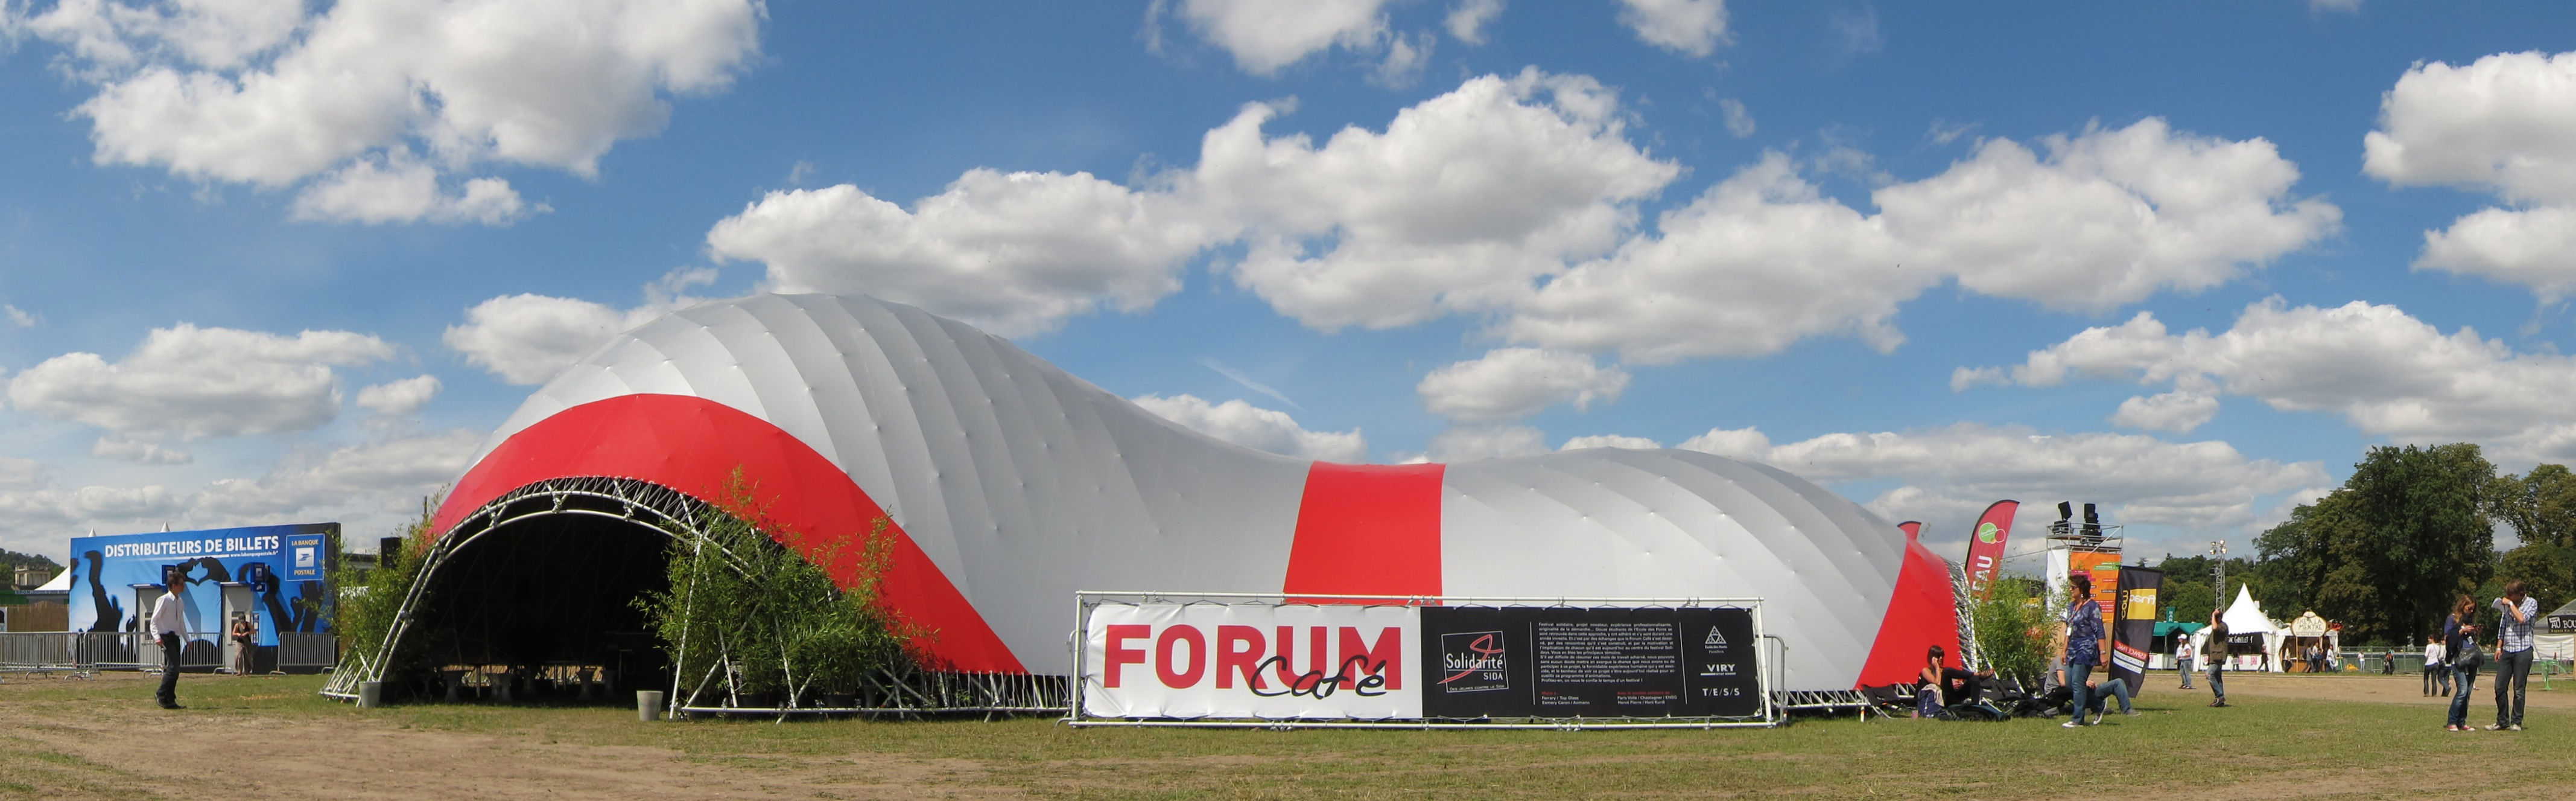
\includegraphics[width=1\textwidth]{solidays.jpg}\label{fig:solidays}}\\
		\subfloat[][Prototype (2007).]{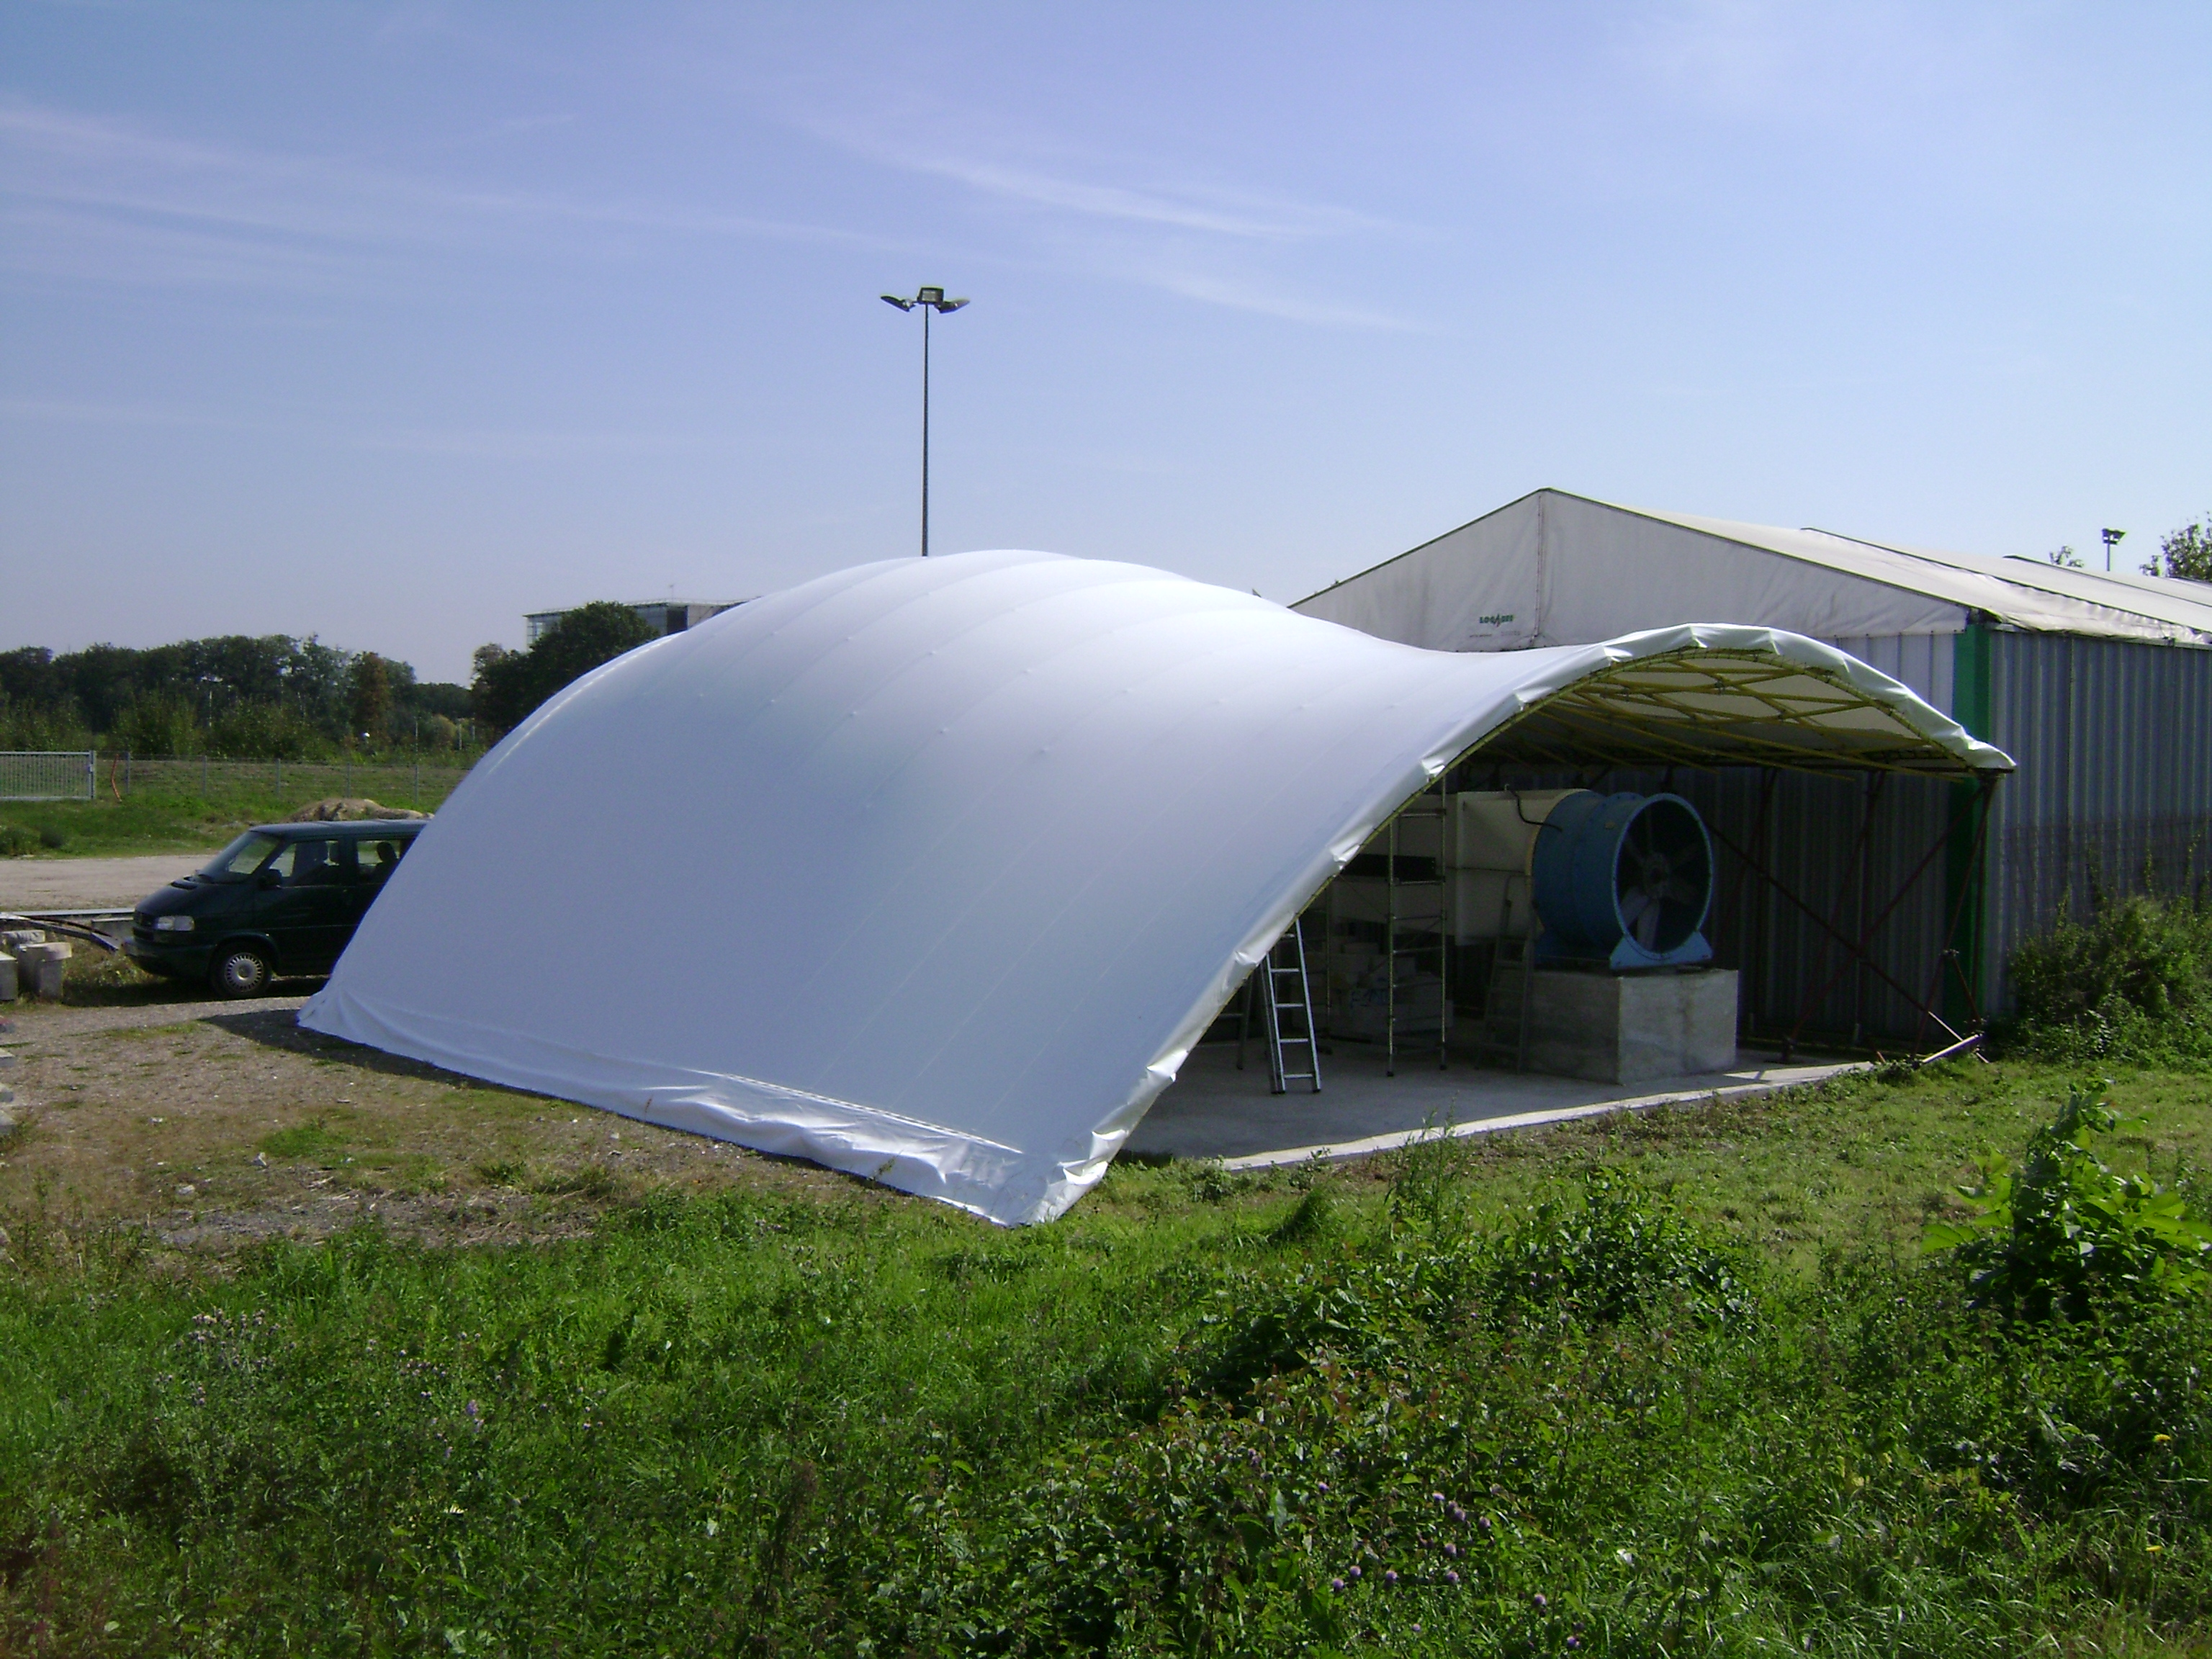
\includegraphics[width=0.48\textwidth]{proto_a.jpg}\label{fig:proto_a}}
		\hspace*{\fill}
		\subfloat[][Prototype (2008).]{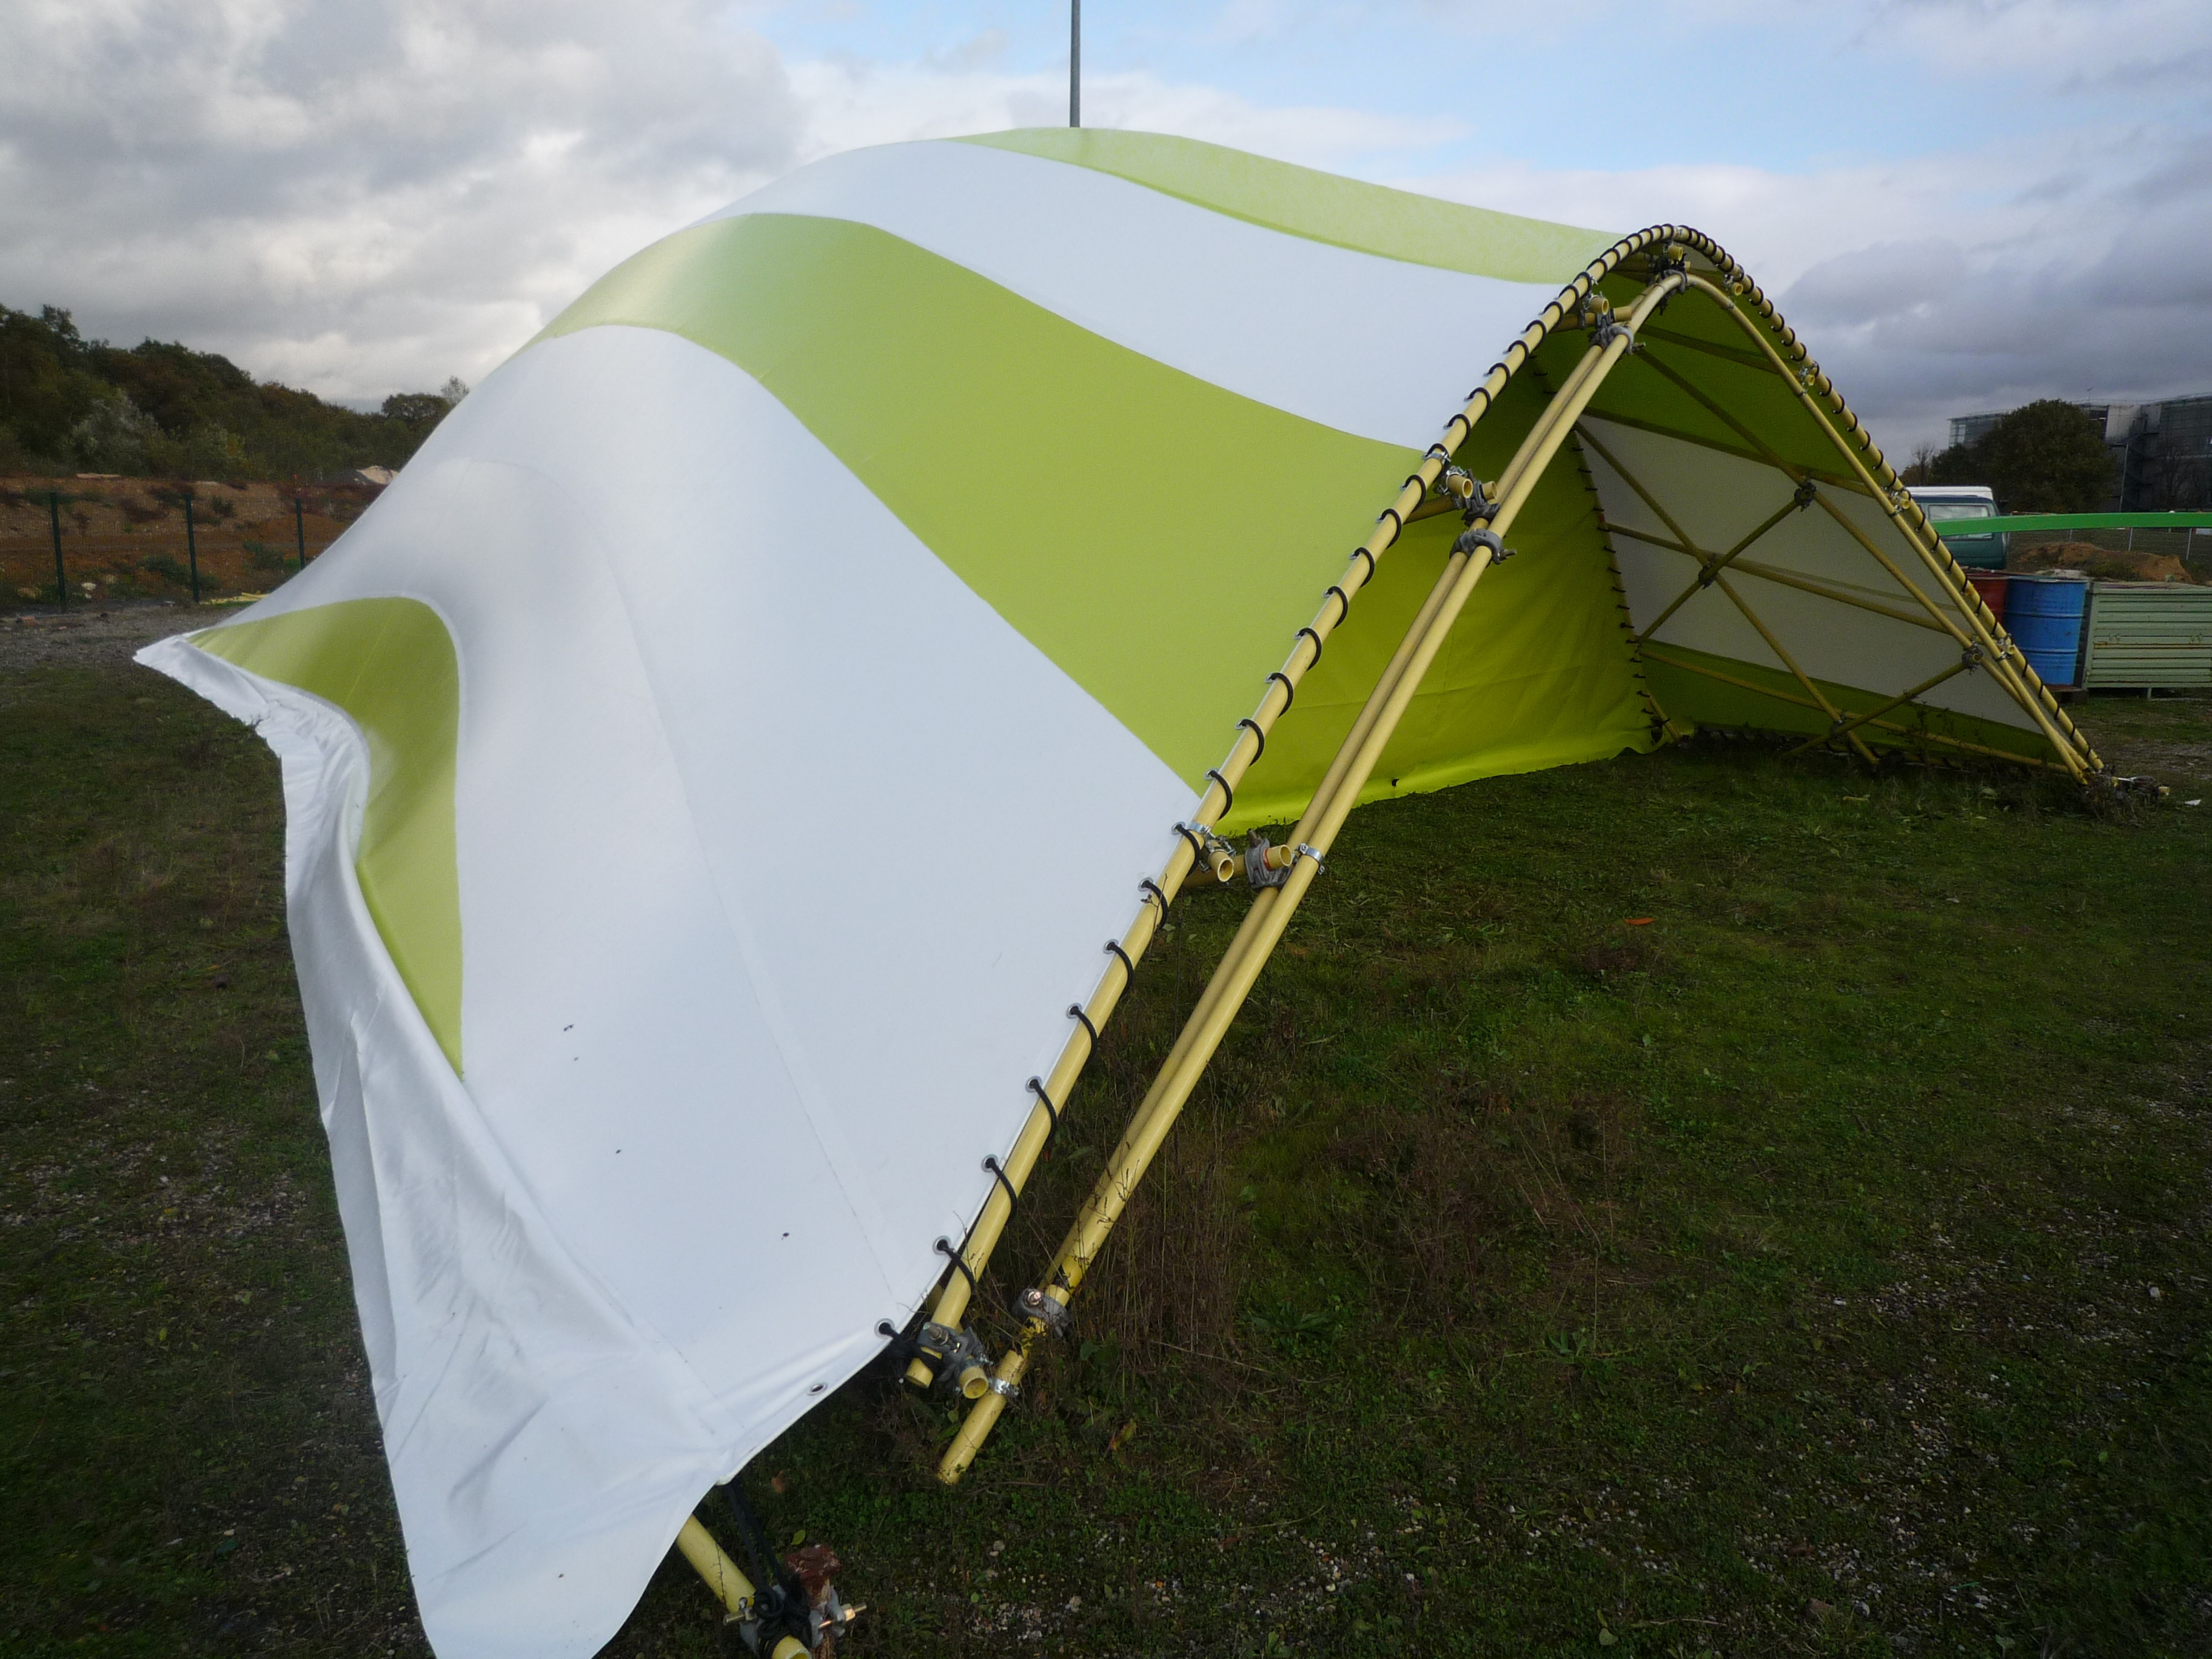
\includegraphics[width=0.48\textwidth]{proto_b.jpg}\label{fig:proto_b}}
		%
		\vspace{10pt}
		\caption{Prototypes and projects of GFRP elastic gridshells.}
		\label{fig:proto}    
\end{figure}

\begin{figure}[p]
	\begin{fullpage}
		\captionsetup[subfloat]{captionskip=10pt}
     		\centering
     		%
		\subfloat[][Mannheim (1975).]{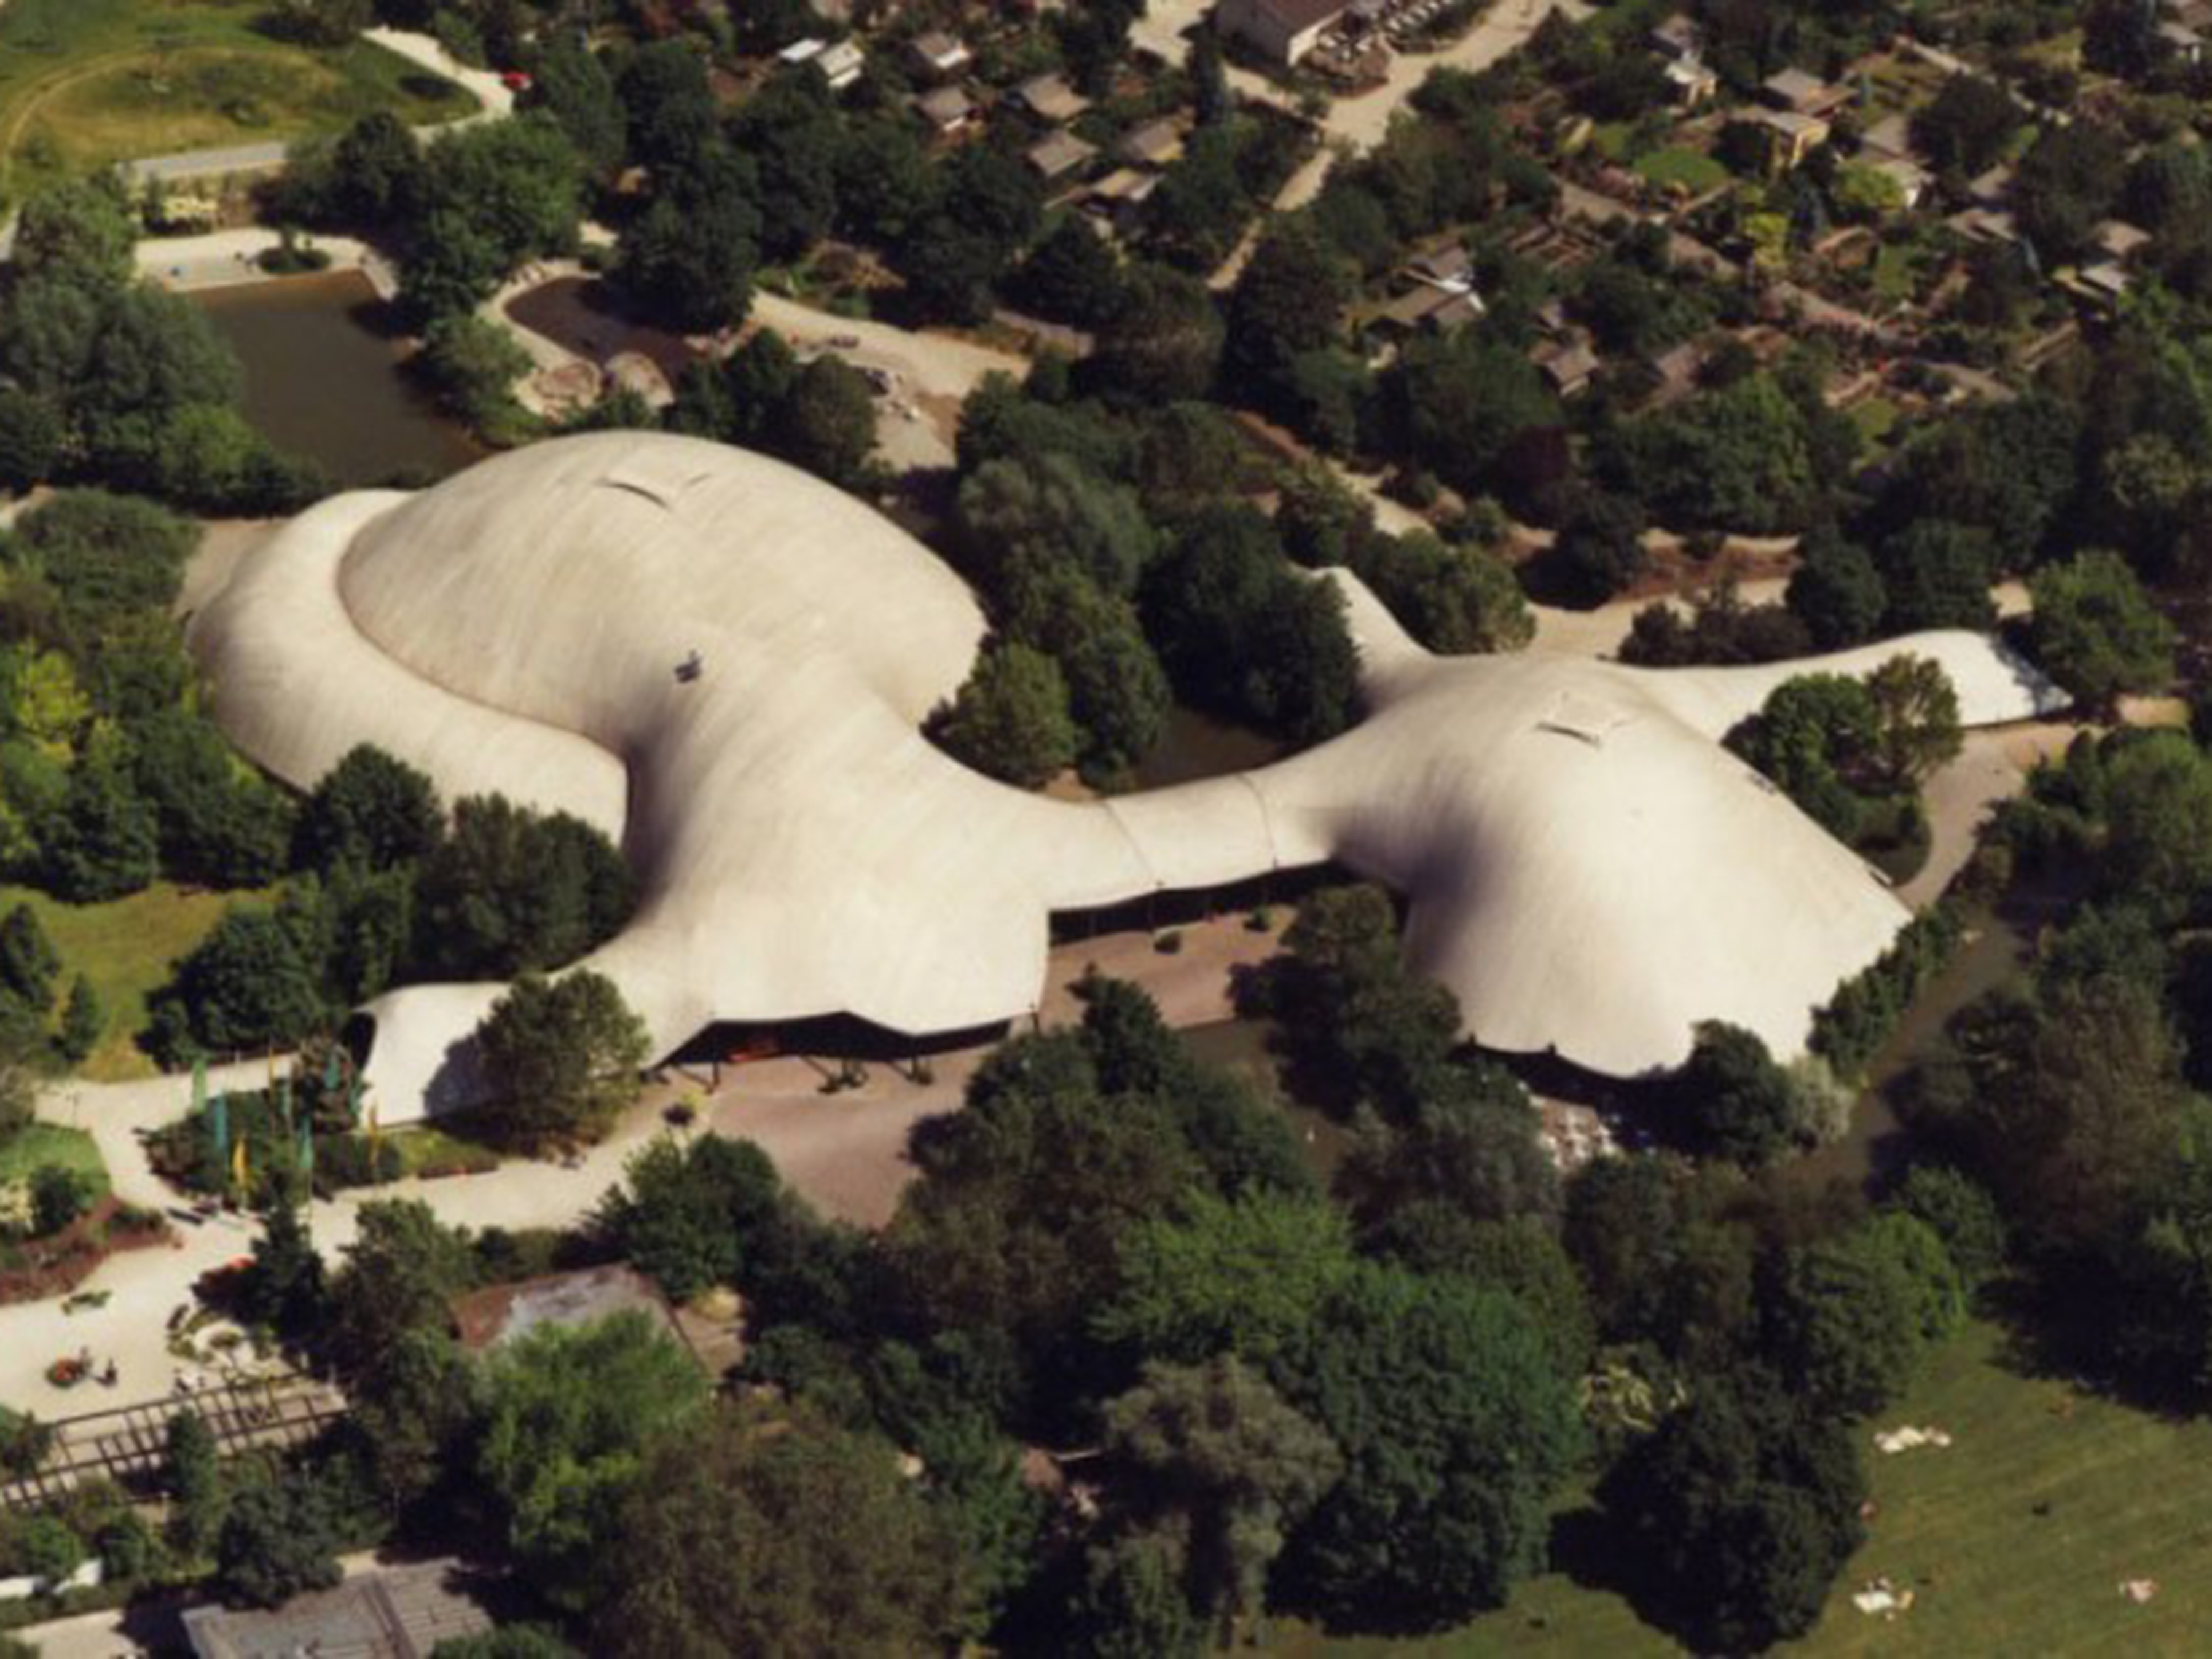
\includegraphics[width=0.48\textwidth]{mannheim_a.jpg}\label{fig:mannheim_a}}
		\hspace*{\fill}
		\subfloat[][Mannheim (1975).]{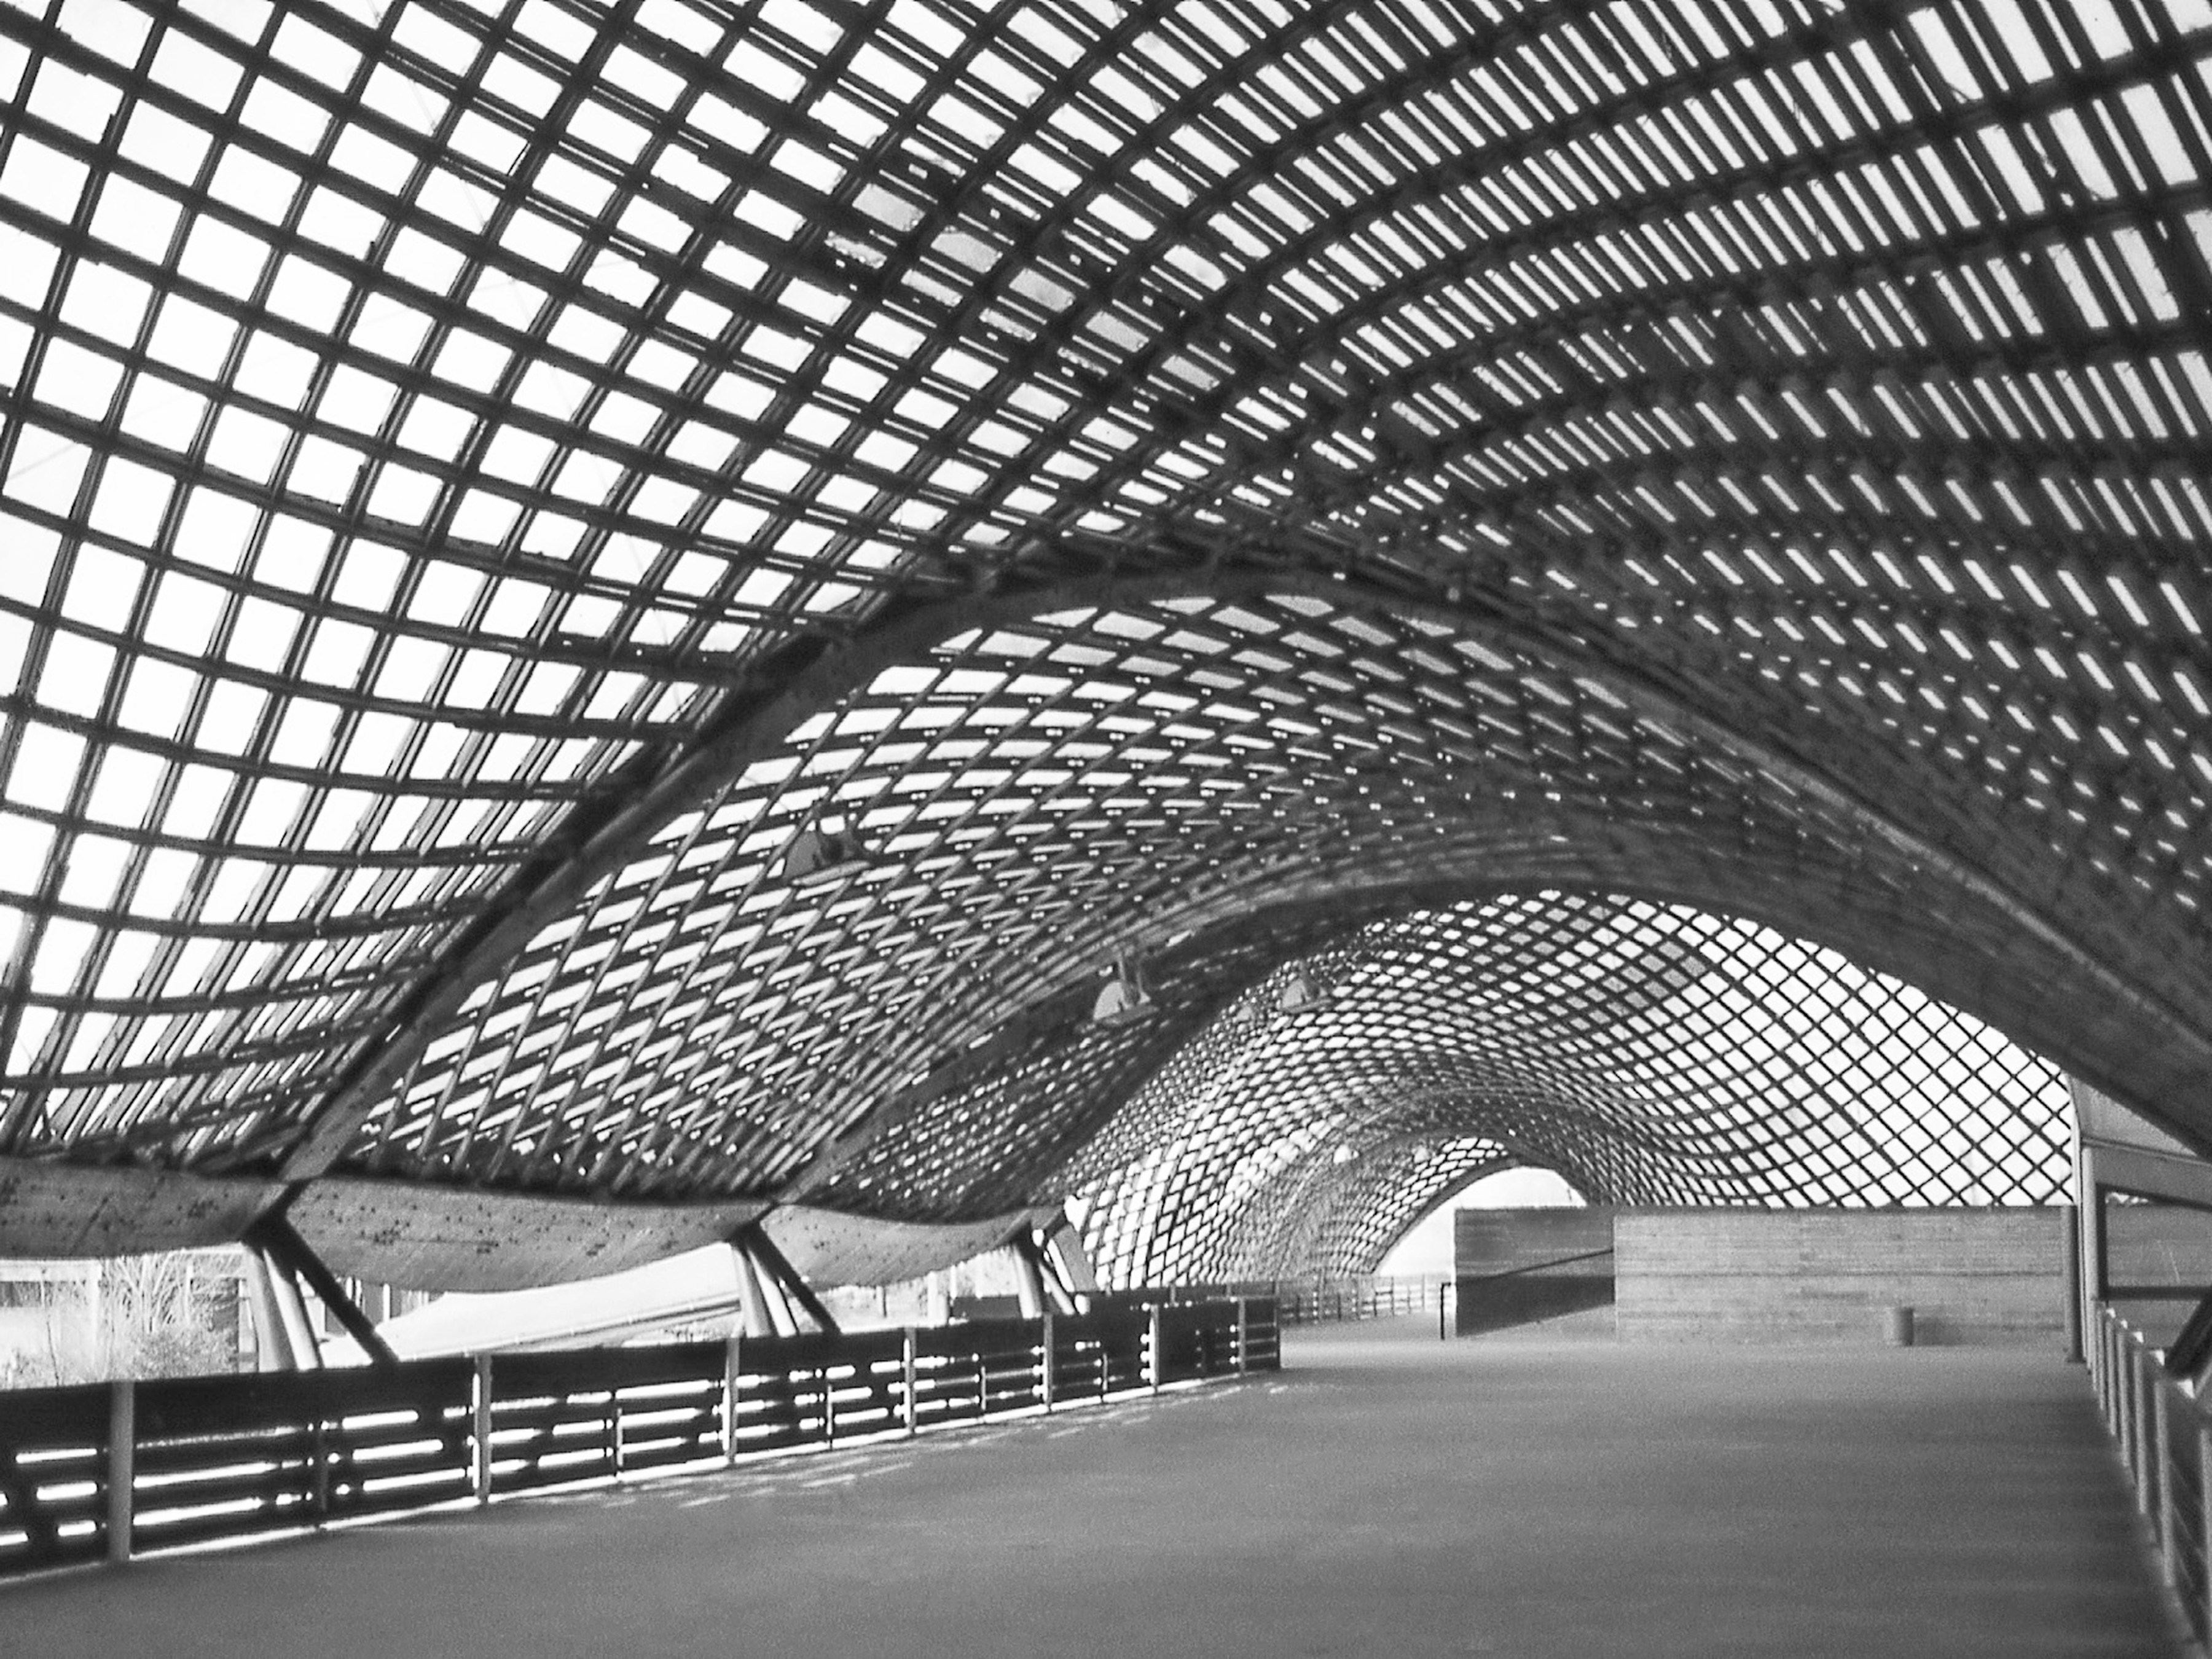
\includegraphics[width=0.48\textwidth]{mannheim_b.jpg}\label{fig:mannheim_b}} \\
		%
		\subfloat[][Downland (2002).]{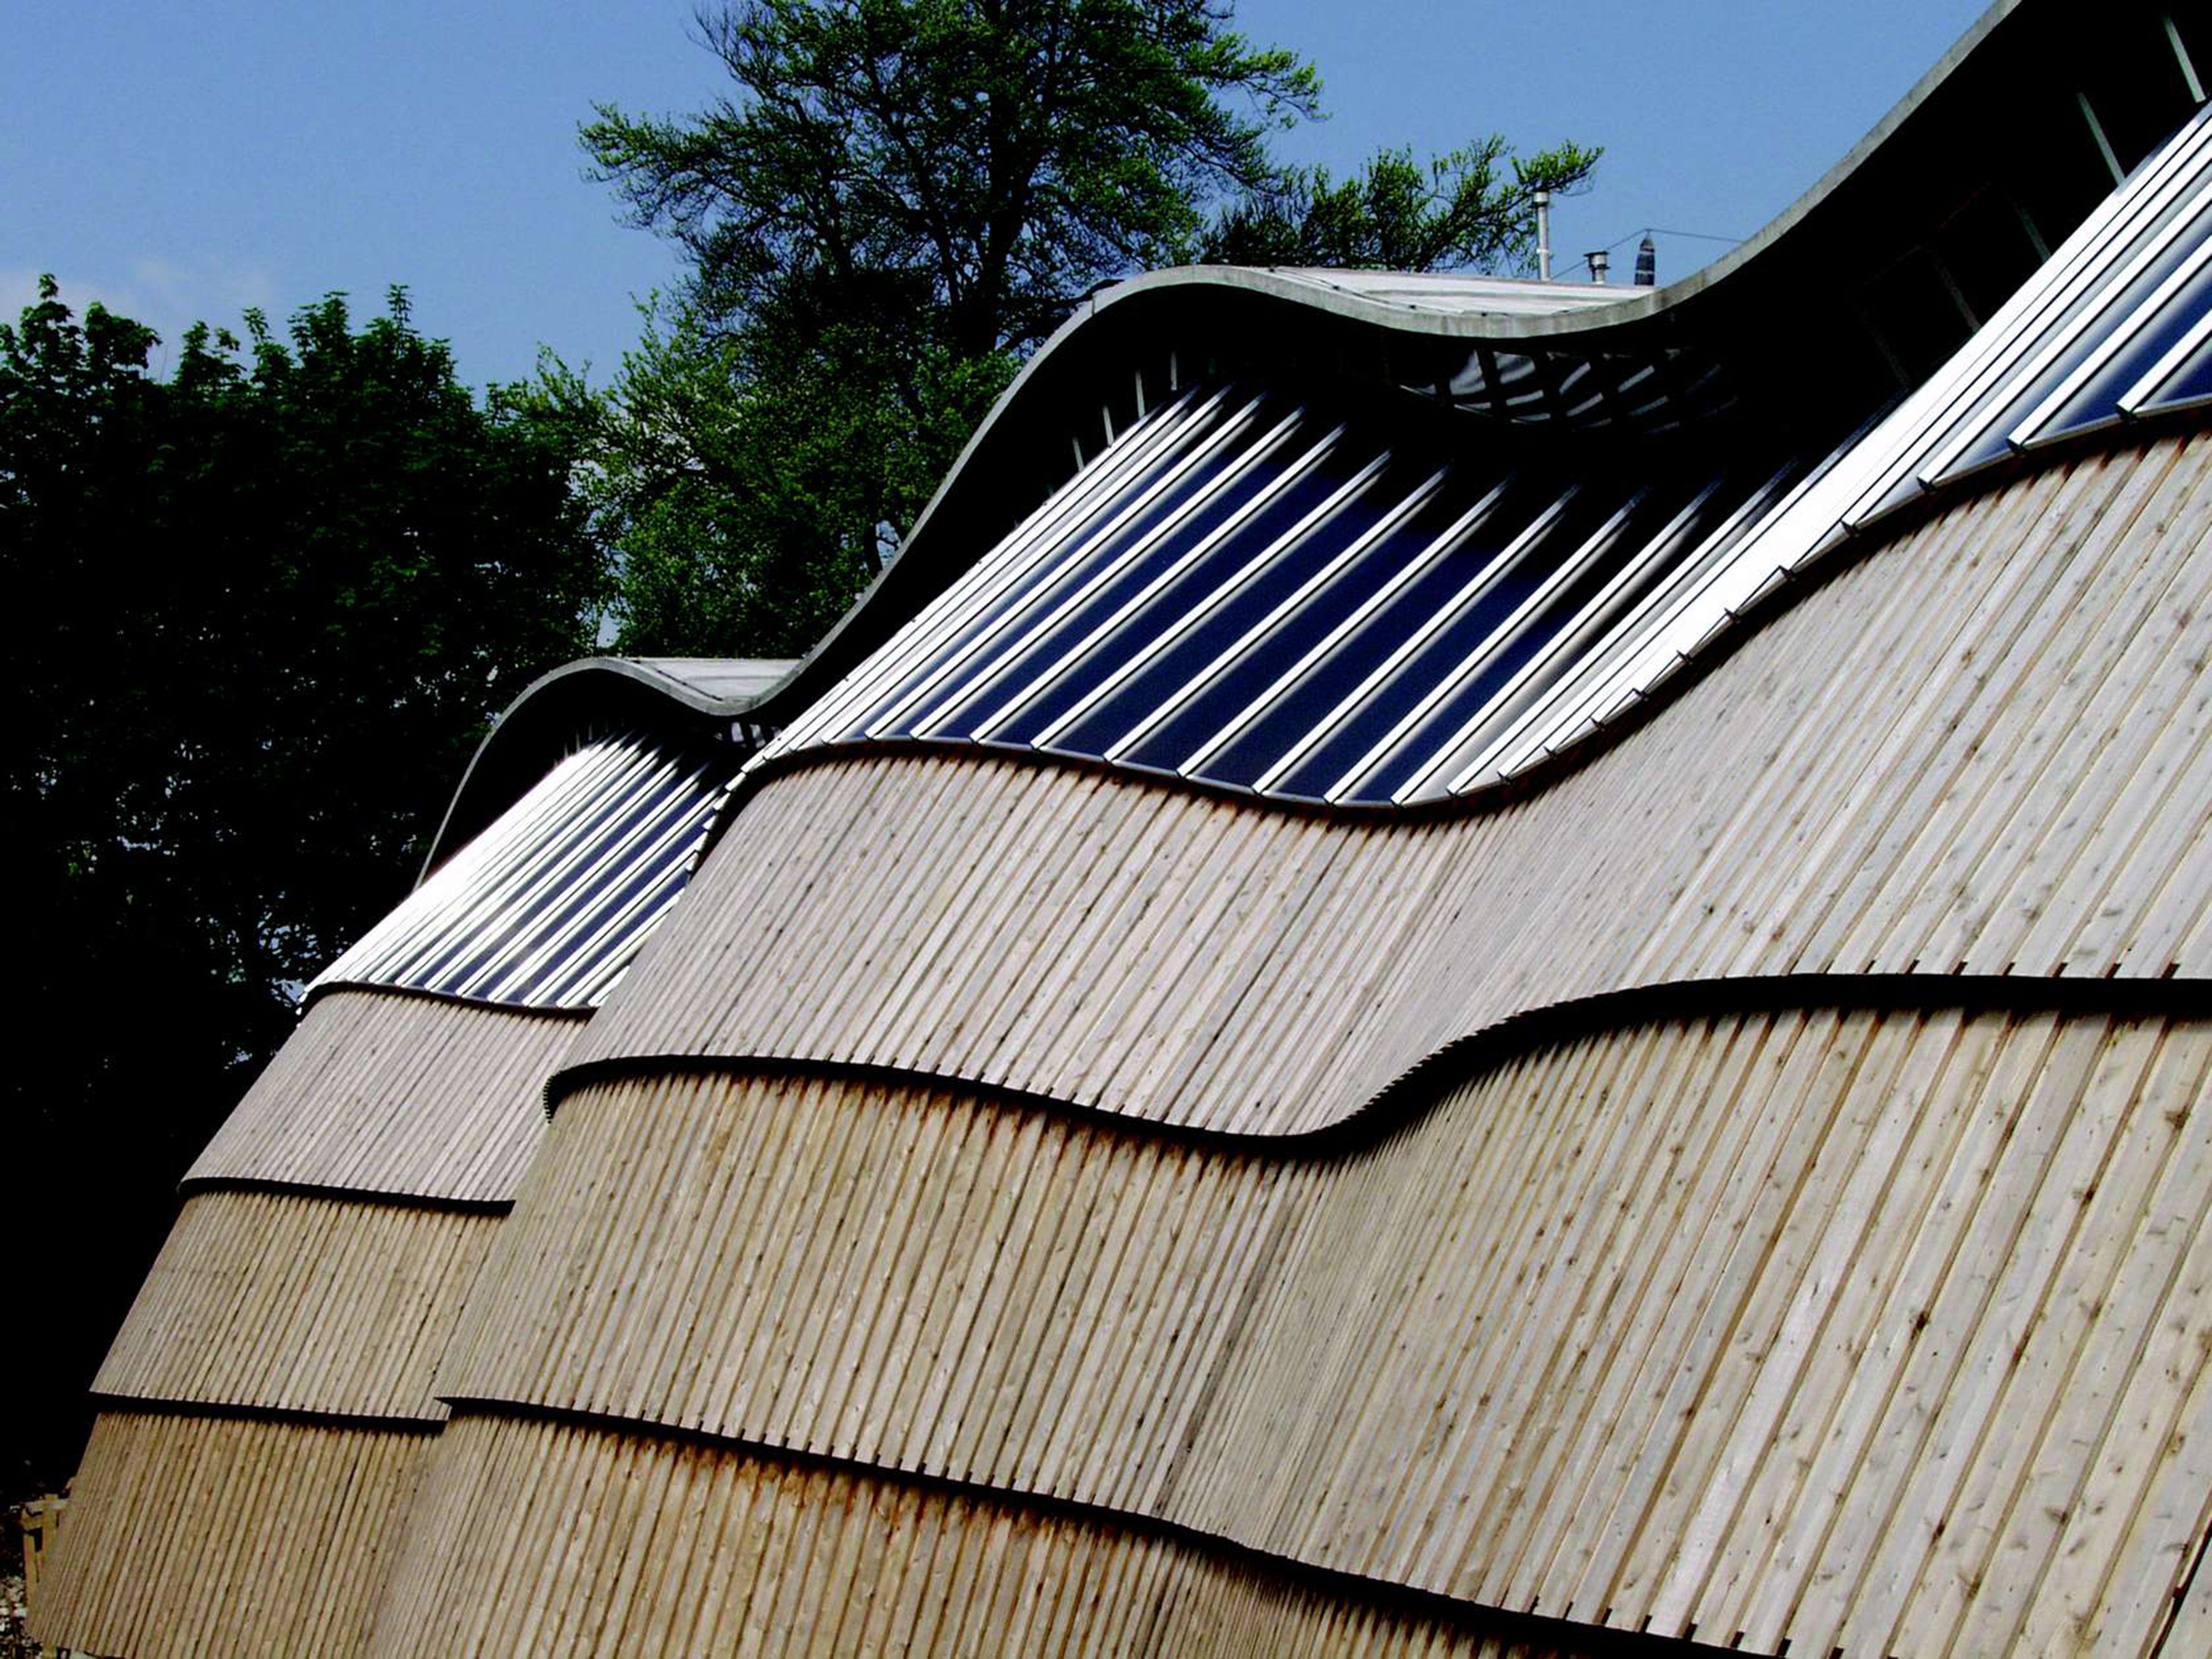
\includegraphics[width=0.48\textwidth]{downland_a.jpg}\label{fig:downland_a}}
		\hspace*{\fill}
		\subfloat[][Downland (2002).]{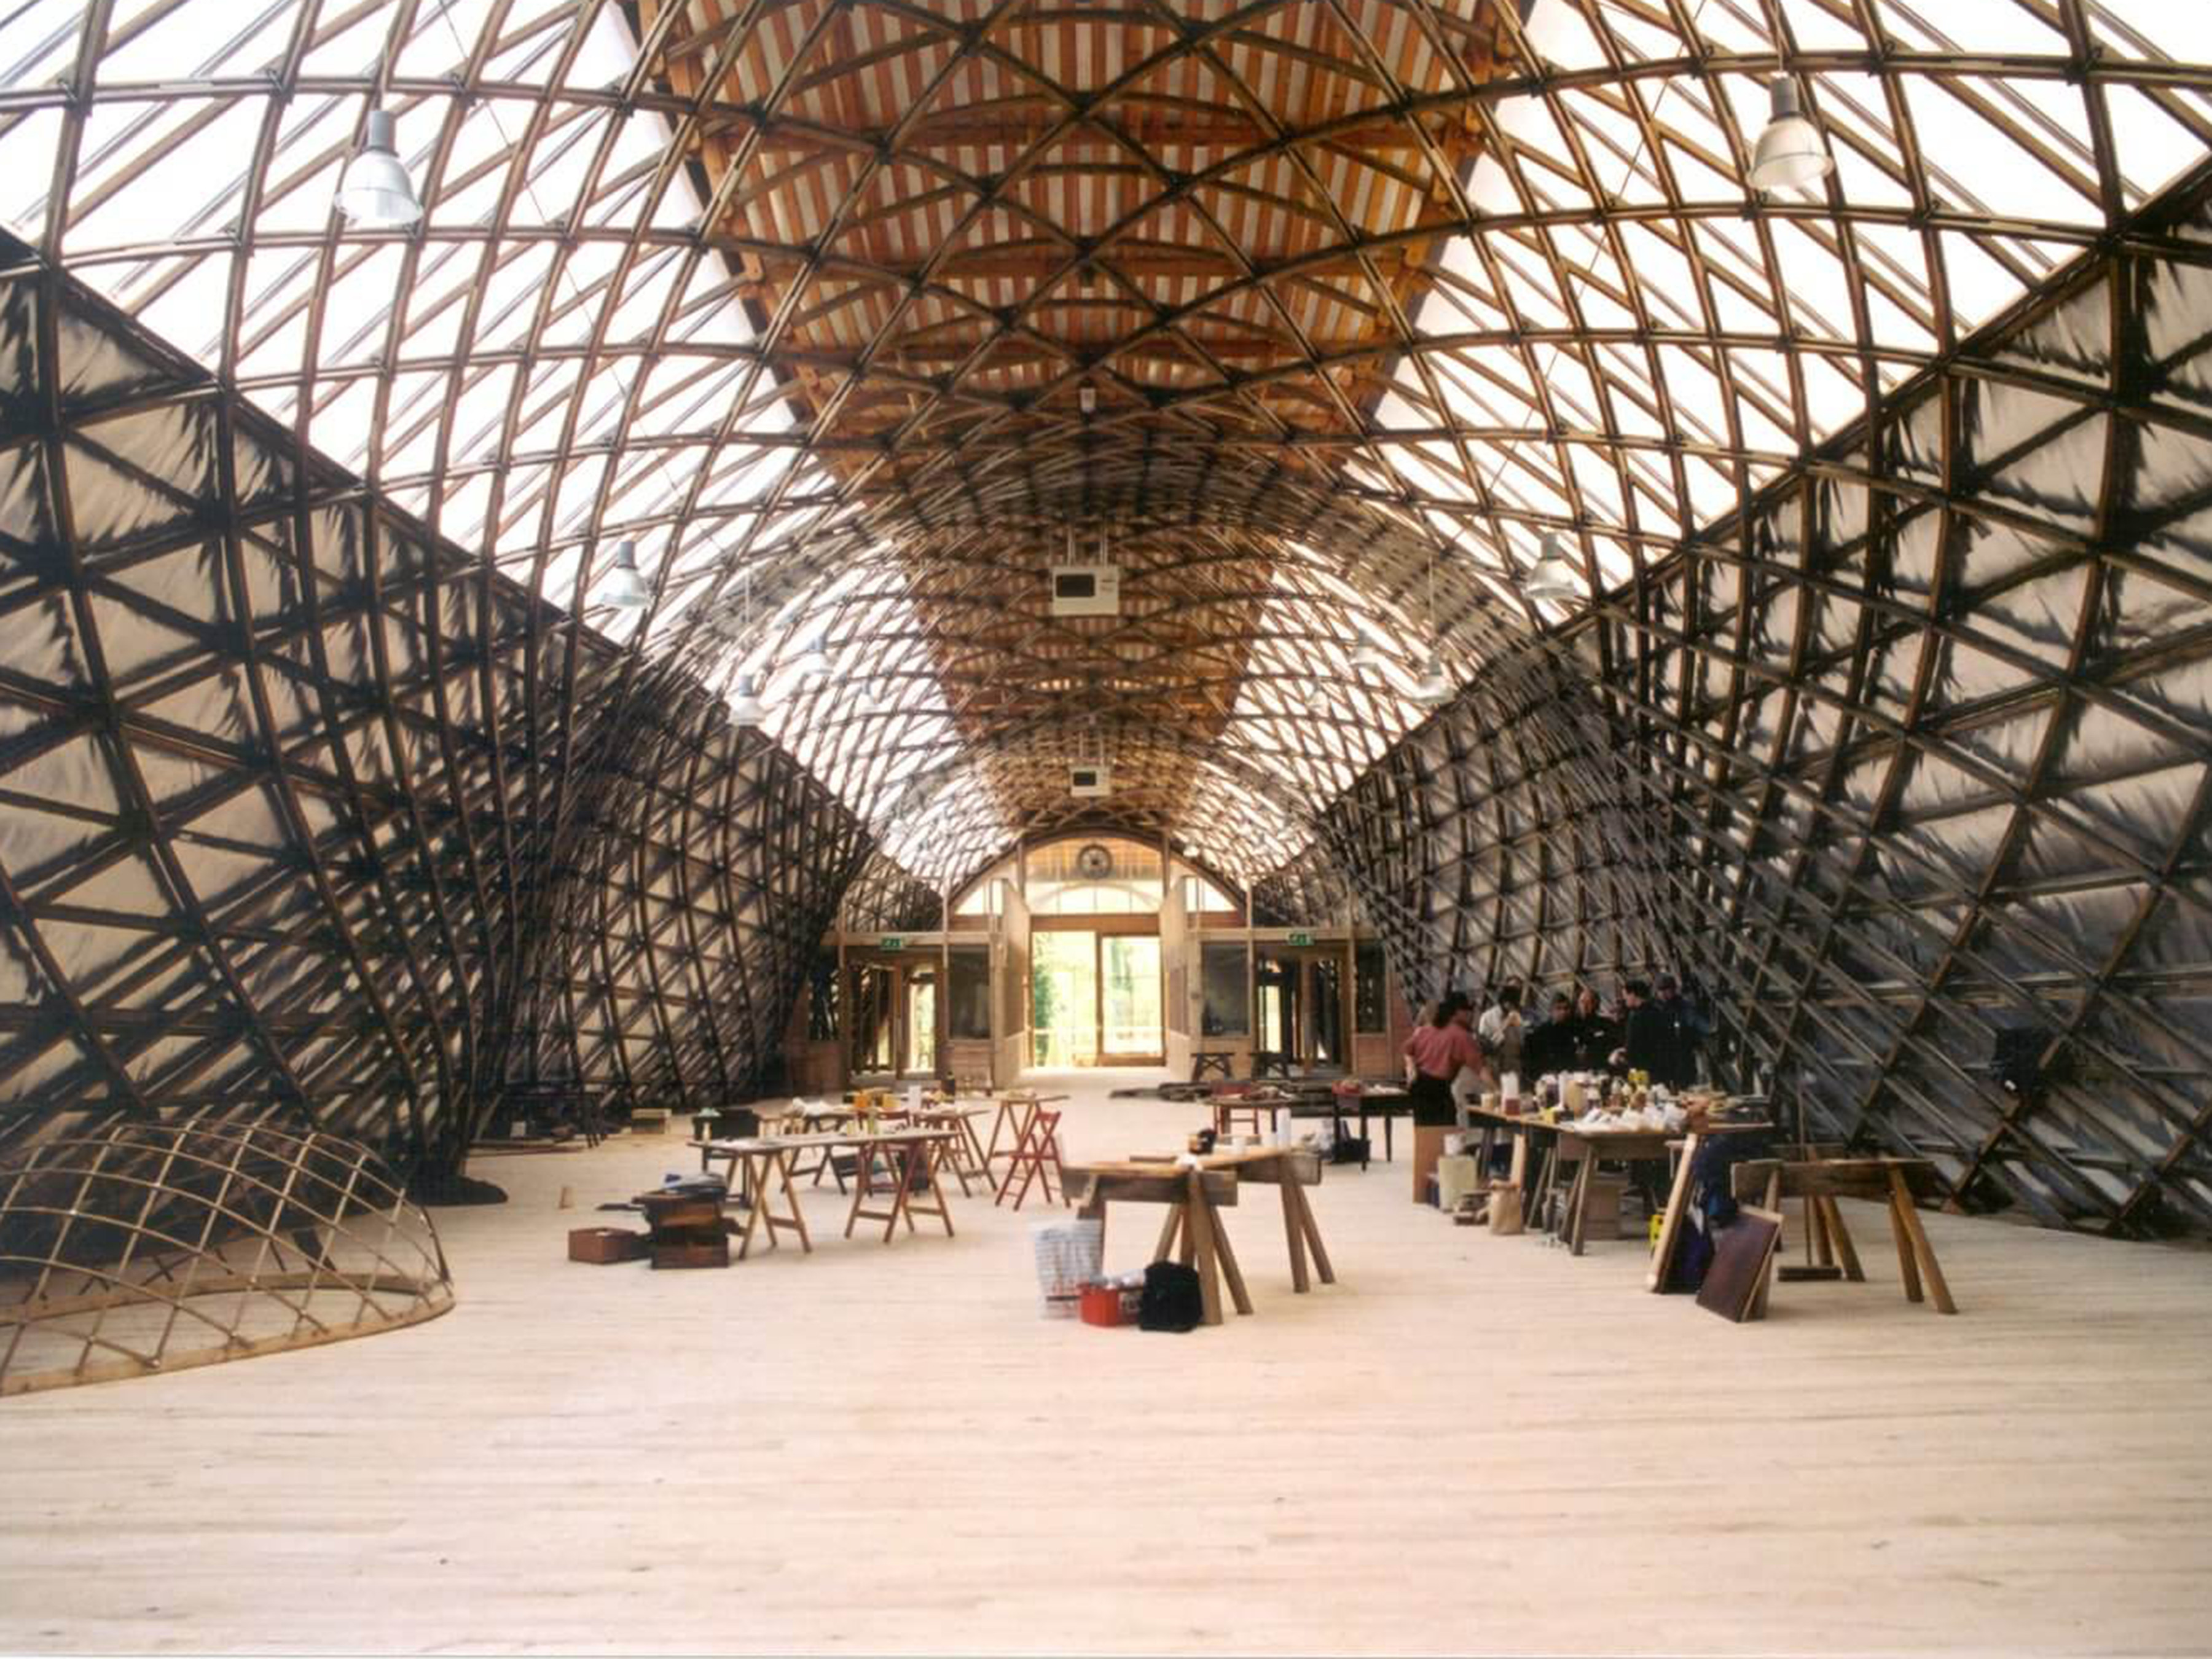
\includegraphics[width=0.48\textwidth]{downland_b.jpg}\label{fig:downland_b}} \\
		%
		\subfloat[][Savill (2006).]{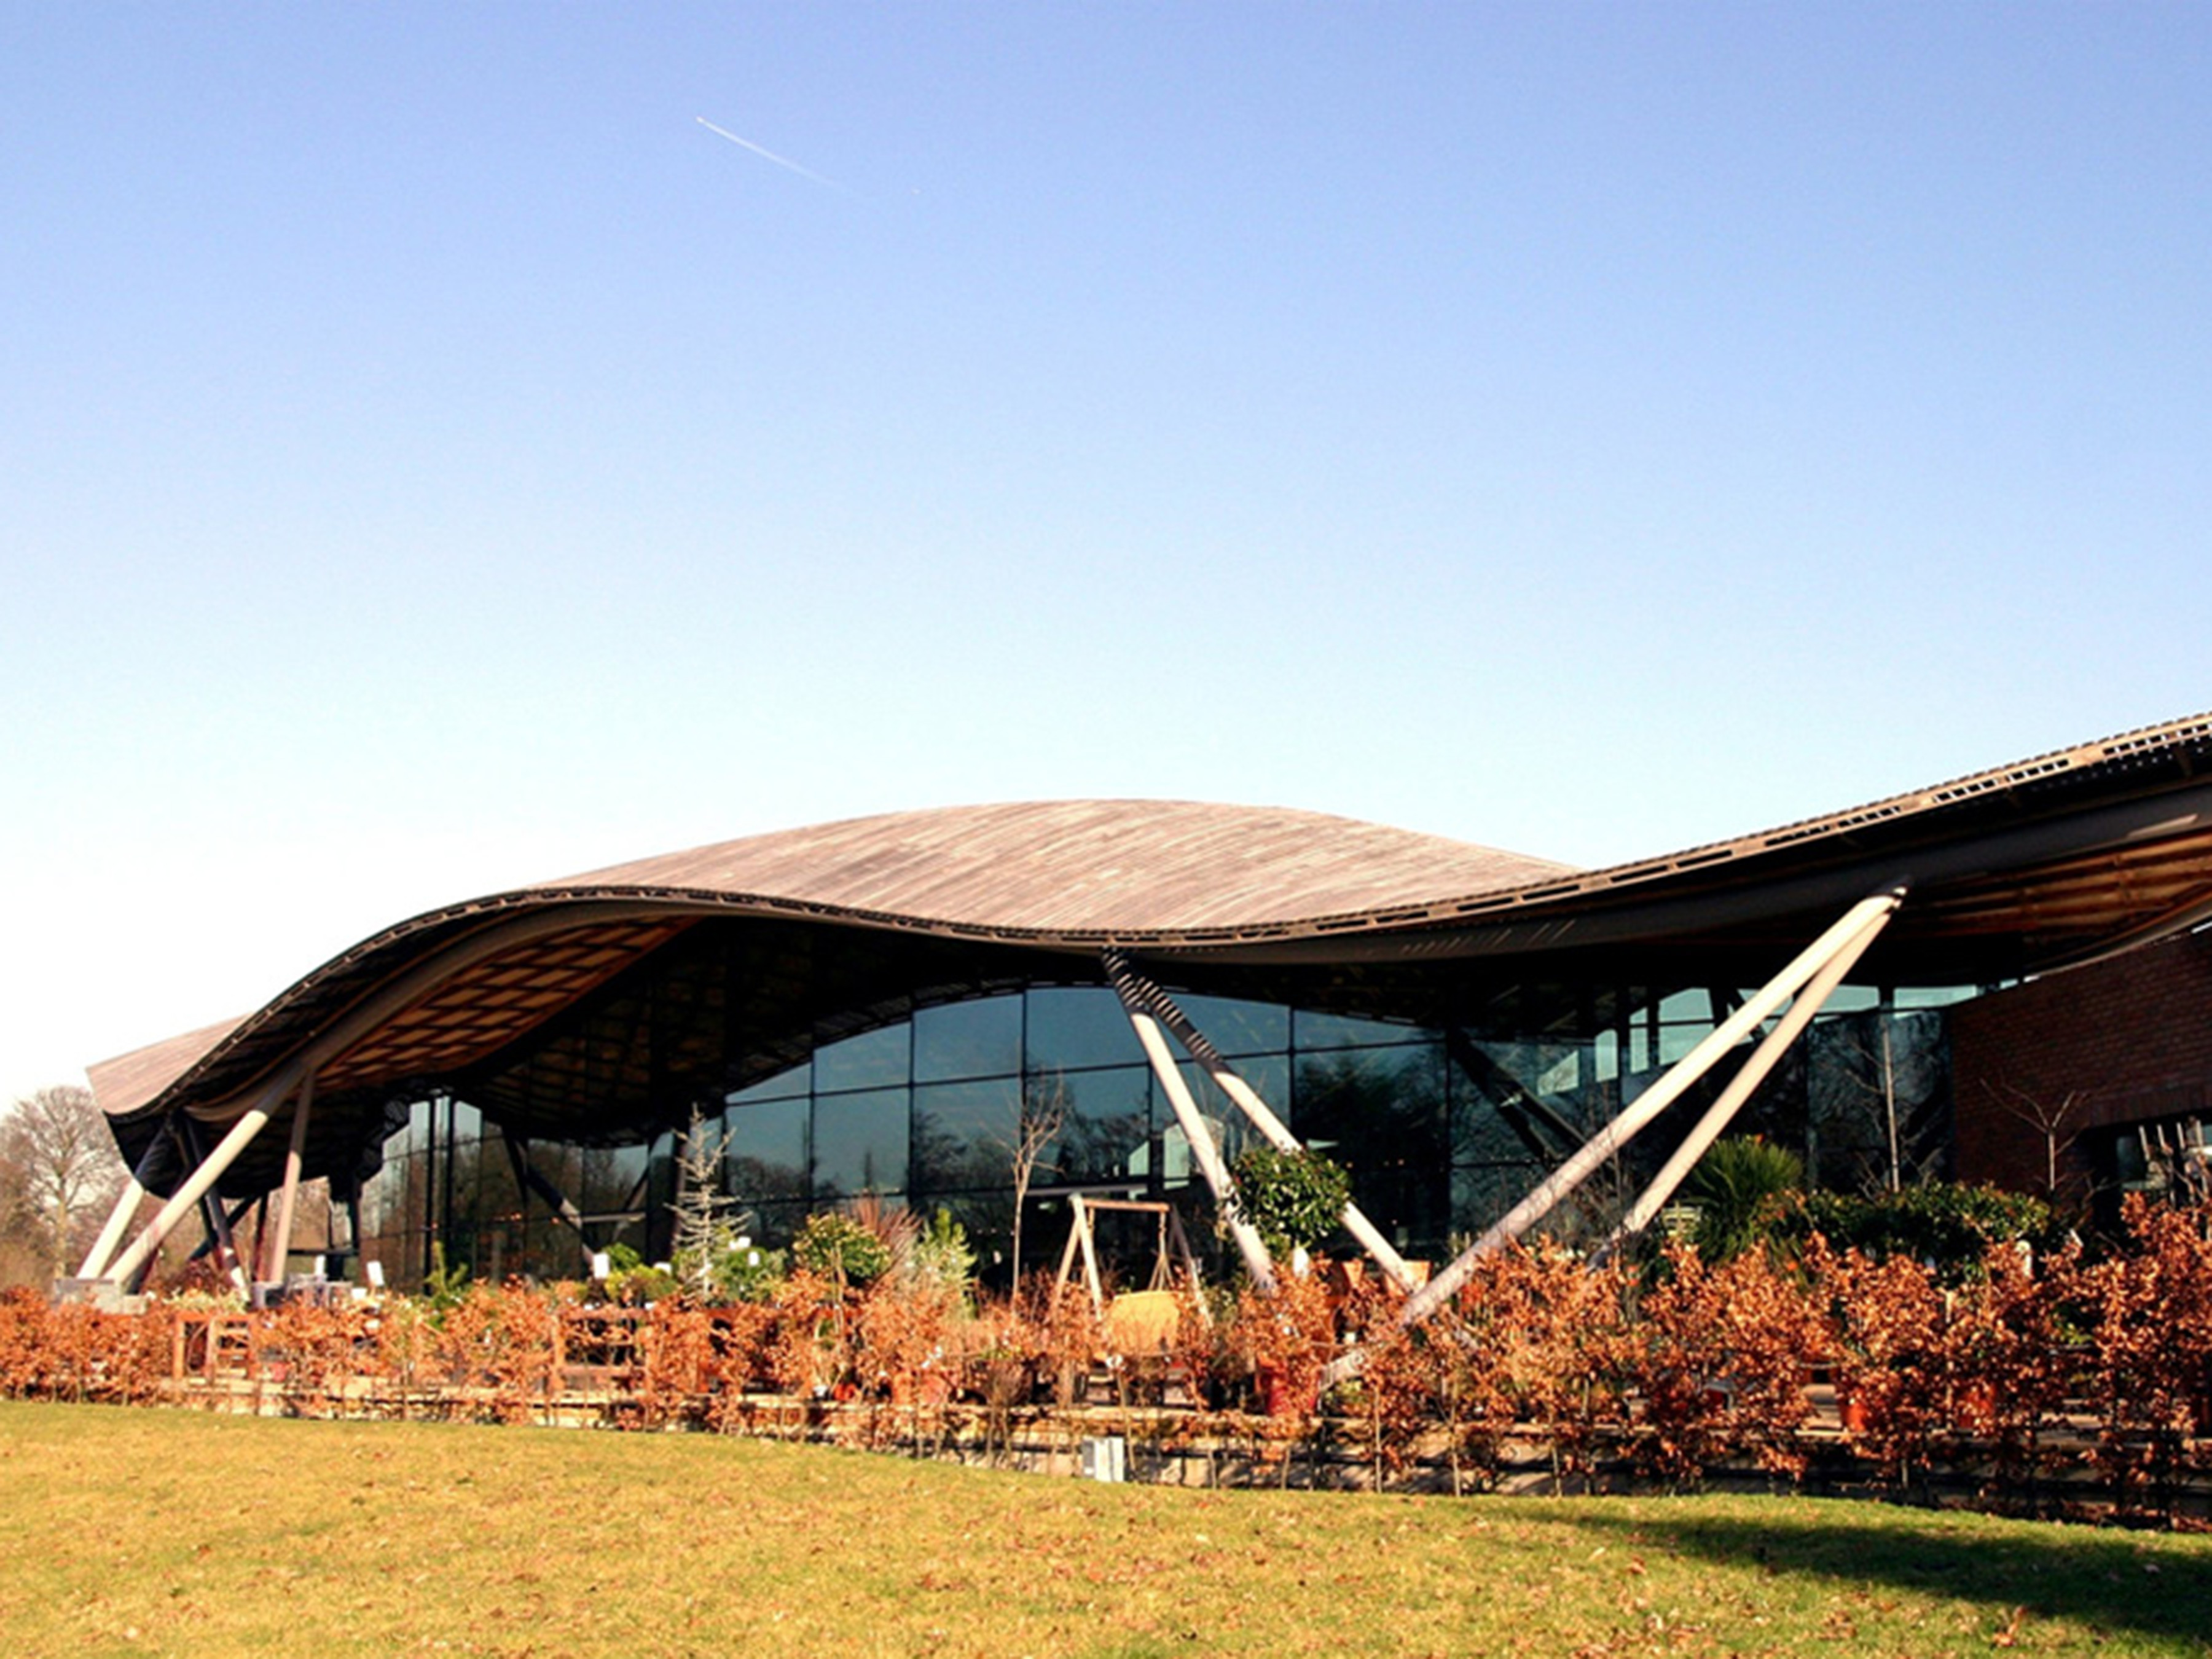
\includegraphics[width=0.48\textwidth]{savill_a.jpg}\label{fig:savill_a}}
		\hspace*{\fill}
		\subfloat[][Savill (2006).]{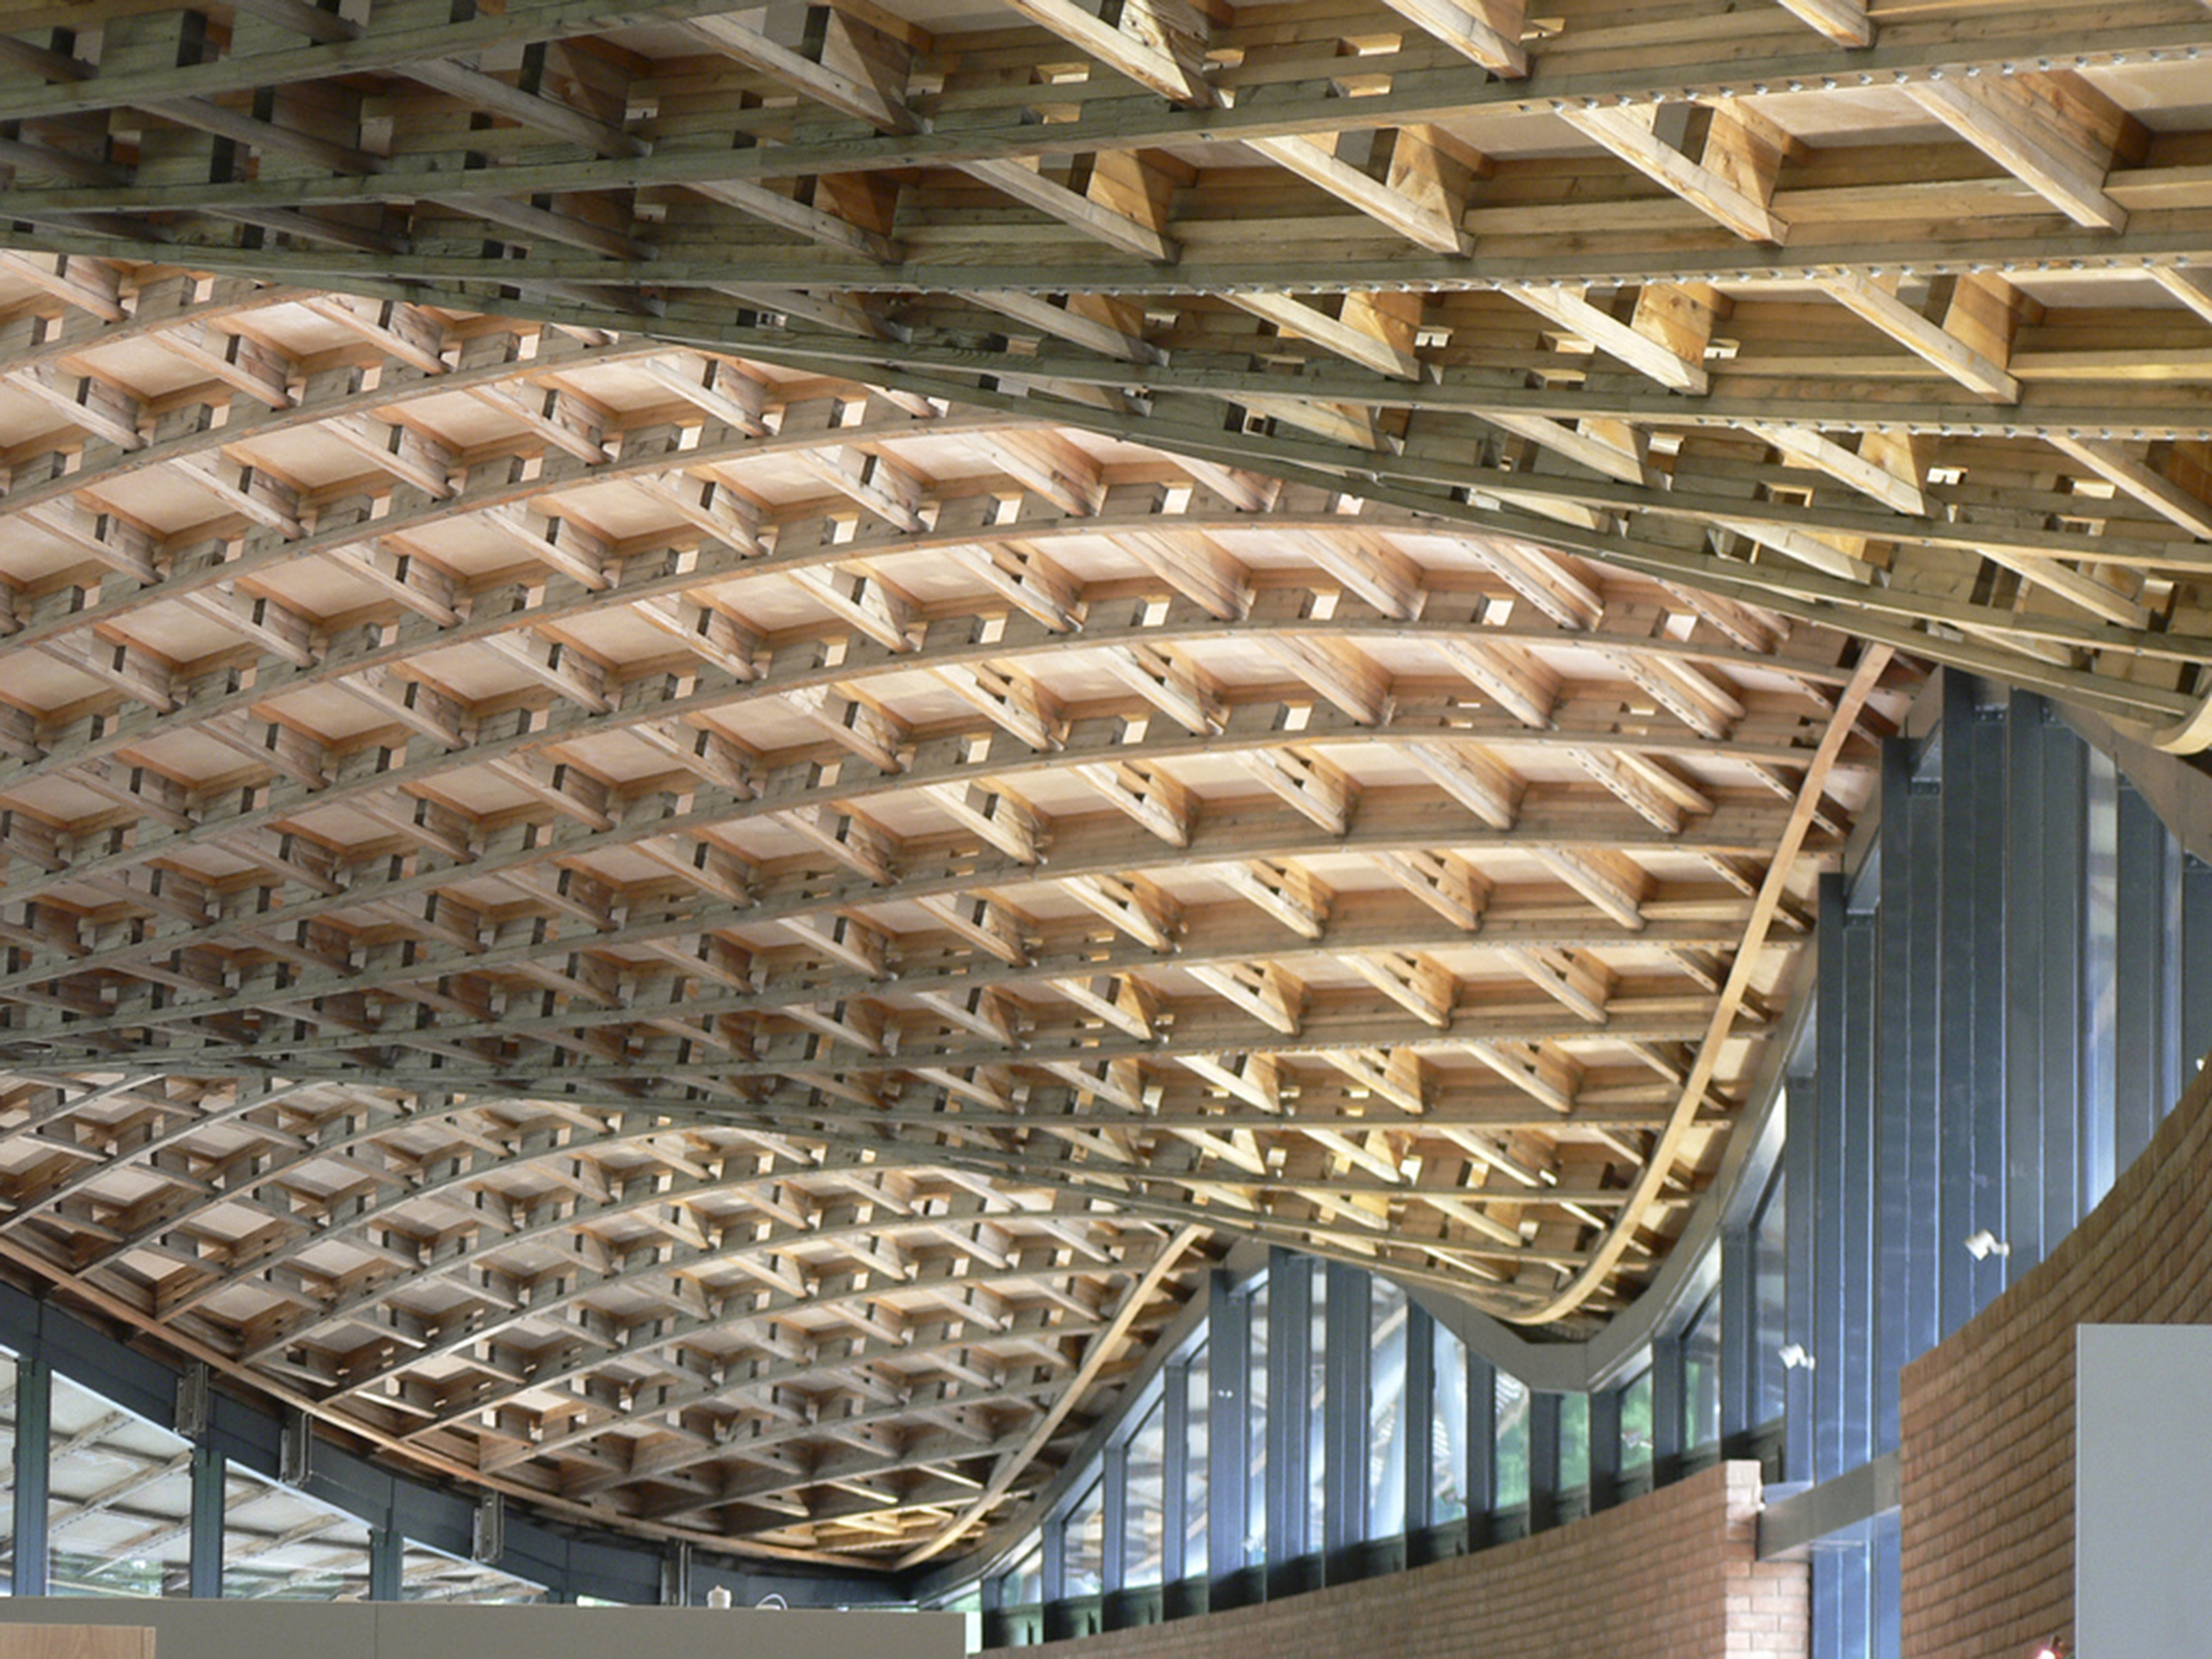
\includegraphics[width=0.48\textwidth]{savill_b.jpg}\label{fig:savill_b}}
		%
		\vspace{20pt}
		\caption{Major permanent projects of elastic wooden gridshells built since 1975.}
		\label{fig:projects}    
	\end{fullpage}
\end{figure}


\section{Elastic gridshells : revisiting Mannheim}


\section{Elastic gridshells : the benefits of composite materials}

Glass fiber reinforced polymer (GFRP) tubes are at the heart of the presented technology. They can favorably replace wood where both resistance and bending ability of the material is sought \cite{Douthe2010}. 

The tubes are made by pultrusion, \enquote{a continuous molding process whereby reinforcing fibers are saturated with a liquid polymer resin and then carefully formed and pulled through a heated die to form a part. Pultrusion results in straight constant cross section parts of virtually any shippable length}.\footnote{Video explaining the pultrusion process~: \url{https://www.youtube.com/watch?v=4MoHNZB5b_Y}} This process is very economic and its standardization guarantees very stable material and mechanical properties. It frees designers from the problem of joining wood pieces with finger joints to obtain long and continuous members and of wood durability.

\begin{figure}[h]
	\centering
		\captionsetup[subfloat]{captionskip=10pt}
		\subfloat[][Forum Café, Solidays (2011).]{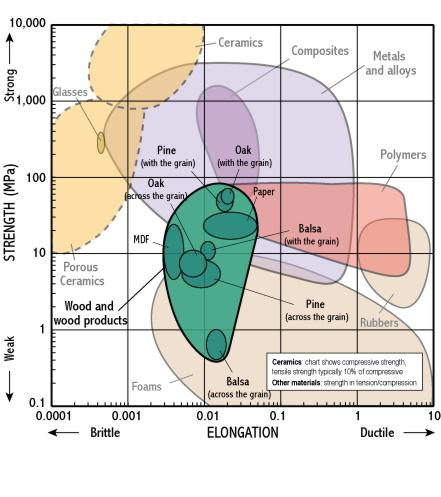
\includegraphics[width=0.6\textwidth]{ashby_woods.jpg}\label{fig:asby_co}}
		\\ \vspace{1cm}
		\subfloat[][Prototype (2007).]{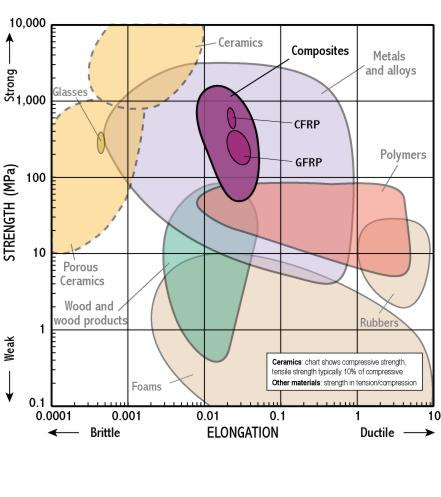
\includegraphics[width=0.6\textwidth]{ashby_composites.jpg}\label{fig:proto_a}}
		%
		\vspace{10pt}
		\caption{Prototypes and projects of GFRP elastic gridshells.}
		\label{fig:proto}    
\end{figure}

\section{Gridshells}

\subsection{Recent projects}
% ------------------------------------------

In 2000, Shigeru Ban innovated by shifting from wooden materials to cardboard for the construction of the Japan Pavilion at the Hanover Expo \cite{McQuaid2006}. More recently, with the development of numerical tools, two new projects were carried out: the wooden gridshells of Downland in 2002 (Weald and Downland Gridshell, Chichester, UK) \cite{Harris2003} and Savill in 2006 (Savill Garden Gridshell, Wick Ln, UK) \cite{Harris2008}. The principles of these projects are similar to that of Mannheim; however, new construction methods were used for the newer gridshells.

The first research works on elastic gridshells are attributed to Frei Otto, founder of the \emph{Institute for Lightweight Structures} (IL, Stuttgart, Germany). Probably one of his first elastic gridshell was built in 1962 with students at Berkley, USA, and was made with steel rods and not wooden elements. During the 60's, he built several experimental structures including one at Essen in 1962 and two at Montreal in 1967 \cite{Liddell2015}. In 1975 he completed the famous Mannheim Multihalle, a wooden shell of \SI{7500 }{m^2}, in collaboration with the engineer Edmund Happold \cite{Happold1975,Otto1976}. This project is generally regarded as the starting point of this new concept.

In 2000, Shigeru Ban innovated by shifting from wooden materials to cardboard for the construction of the Japan Pavilion at the Hanover Expo \cite{McQuaid2006}. More recently, with the development of numerical tools, new projects were carried out~: the wooden gridshells of Downland, UK, in 2002 \cite{Harris2003} and Savill, UK, in 2006 \cite{Harris2008}. The principles of these projects are similar to that of Mannheim. However, new construction methods were used for the newer gridshells. The flat lattice of the Downland gridshell was built on a modular scaffold platform, which height was altered progressively to deform the lattice. The grid was braced by a third direction of laths. The lattice of the Savill gridshell was built on a fixed scaffold platform. Small jacks where used to deform the lattice, pushing from below. The grid was then braced with plywood panels, which also served as the first cladding layer. 

The Orangery roof at Chiddingstone Castle is a smaller gridshell built in 2006. The lattice is very similar to the one employed in Downland. But this time the grid is braced with a diagonal cable network and the cladding is made of triangular glass panels (the first of this kind). To this end, the steel connection includes a cable clamping system and is equipped with a threaded hole to accept fixing parts for the glazing.




\subsection{Recent developments}
% ------------------------------------------
Based on this groundwork, the Navier laboratory has developed a research program on gridshells for the last decade, focusing on both the use of new materials and the development of more efficient numerical methods \citep{Douthe2007}. These developments have been validated by the construction of two prototypes (Figures \ref{fig:4}a and \ref{fig:4}b) whose areas were about 150 m\textsuperscript{2}.


In 2011, the laboratory used its expert knowledge for a large-scale project \citep{Baverel2012}, the forum of the Solidays festival (\autoref{fig:4}c). This achievement, built by voluntary workers, has been the first composite material gridshell to house public.

In 2012, the context is favorable for a new achievement named \emph{"Temporary Cathedral of Créteil"}. Although this gridshell has an area very similar to the Solidays one, the project raised new challenges, in particular the challenge of reliability. Indeed, its period of use is at least two years. Additionally, the skills coming from T/E/S/S company made possible important developments such as for doors, lacing edge beam, anchorages and sleeves.

Unlike the two first prototypes, the gridshells built for Solidays and at Créteil are based on a new approach regarding shape-structure relationship. Indeed, thanks to a numerical tool performing the compass method, the geometry of the object is no longer defined as the reversal of a hanging net – in this case, only the flat geometry could be mastered \citep{Addis2013} – but now the flat geometry is straight deducted from the one proposed by the architect.
This new approach opens up new architectural horizons, making possible the exploration of new shapes for gridshells.

The Faraday Pavilion : \cite{Nicholas2013}
The Pishwanton / lothian : \cite{Pishwanton2003}
The laboratory Navier tested various numerical methods to generate such grids \citep{Bouhaya2009}
Masson :  \cite{Masson2017}.
\begin{figure}[t]
	\centering
		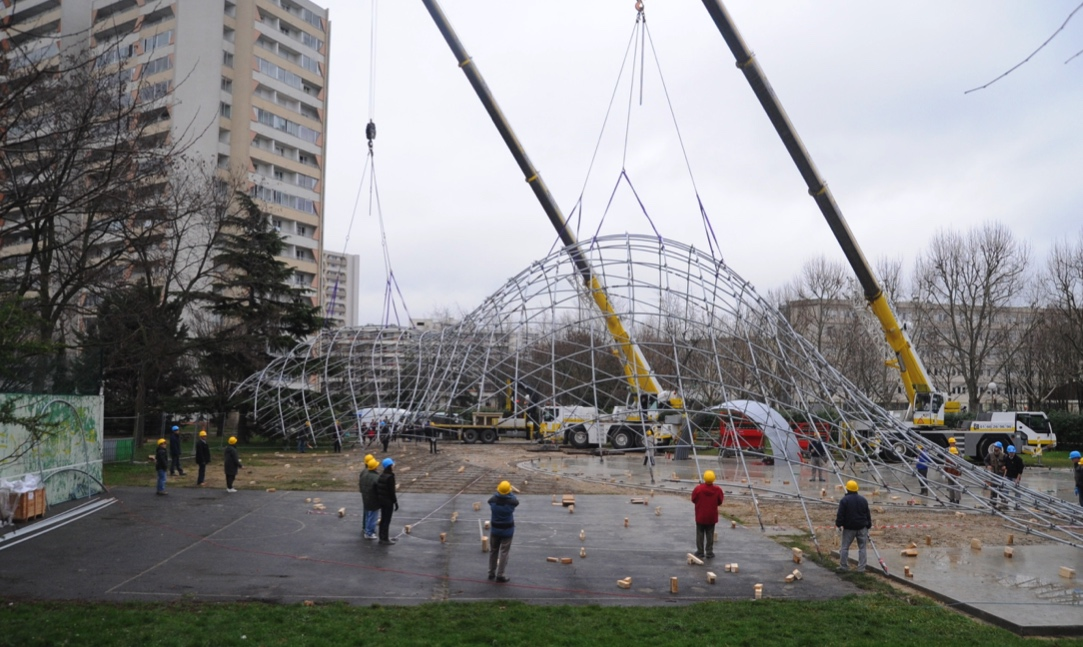
\includegraphics[width=\textwidth]{image6}
	\caption{Erection of the primary grid by two cranes}
	\label{fig:5}
\end{figure}


\subsection{Gridshell in composite material}
% ------------------------------------------

The benefits of GFRP gridshells have been covered previously. We just recall the main aspects.

The gridshells built in composite material, being at the heart of this paper, are consistent with the framework defined previously, that is to say :


Glass fiber reinforced polymer (GFRP) tubes are at the heart of the presented technology. They can favorably replace wood where both resistance and bending ability of the material is sought \cite{Douthe2010}. 

The tubes are made by pultrusion, \enquote{a continuous molding process whereby reinforcing fibers are saturated with a liquid polymer resin and then carefully formed and pulled through a heated die to form a part. Pultrusion results in straight constant cross section parts of virtually any shippable length}.\footnote{Video explaining the pultrusion process~: \url{https://www.youtube.com/watch?v=4MoHNZB5b_Y}} This process is very economic and its standardization guarantees very stable material and mechanical properties. It frees designers from the problem of joining wood pieces with finger joints to obtain long and continuous members and of wood durability. 


\subsubsection{Structural Typology}
% ------------------------------------------
Their mechanical behaviour is very similar to the one of real shells even if the material is discrete and located in a grid more or less open. In spite of that, gridshells benefit from the same advantages as the ones showed by an eggshell : they can cross large span using a low amount of material. Their stiffness is mainly linked to their double-curved shape.


\subsubsection{Material Flexibility for Structural Rigidity}
% ------------------------------------------
In this field of application, composite materials like glass fibre reinforced polymer (GFRP) could favourably replace wood, where both resistance and bending ability of the material is sought \citep{Douthe2010}. The stiffness of the structure does not derive from the intrinsic material rigidity but principally from its geometric curvature. Ideally, the composite profiles are produced by pultrusion, an economic continuous moulded process. The standardization of the process guaranties very stable material and mechanical properties. It frees designers from the painful problematic of wood joining and wood durability. The characterization of this material is presented further in the paper.


\subsubsection{Erection Process}
% ------------------------------------------
Usually, the grid morphology is not trivial and leads to design numerous costly and complex joints. To overcome this issue, an original and innovative erection process was developed that takes advantage of the flexibility inherent to slender elements. A regular planar grid made of long continuous linear members is built on the ground (\autoref{fig:6}a). The elements are pinned together so the grid has no in-plane shear stiffness and can accommodate large-scale deformations during erection. Then, the grid is bent elastically to its final shape (\autoref{fig:5}). Finally, the grid is frozen in the desired shape with a third layer of bracing members (\autoref{fig:6}b) and the structure becomes a shell.
\begin{figure}[t]
	\begin{minipage}[b]{.70\linewidth}
		\centering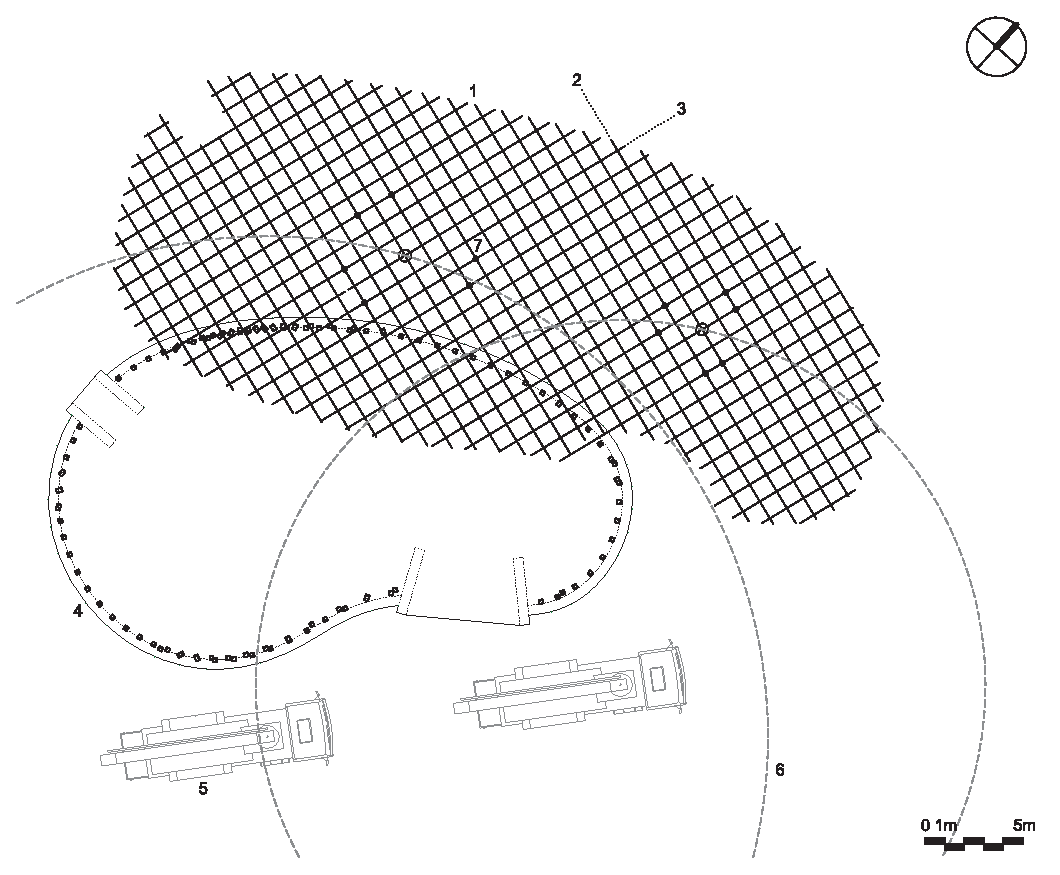
\includegraphics[width=0.95\textwidth]{image5}
	\end{minipage} \hfill
	\begin{minipage}[b]{.25\linewidth}
		\centering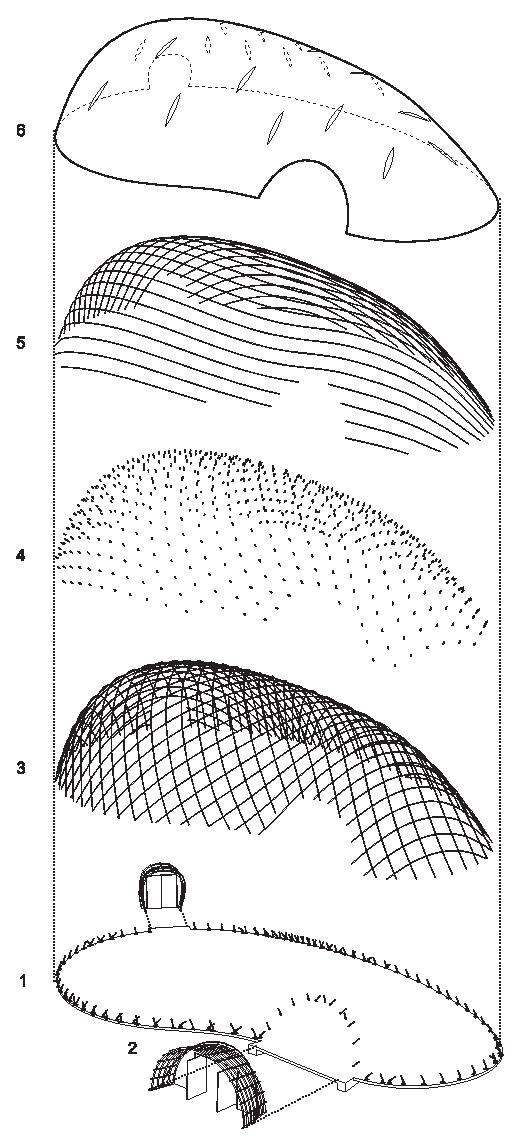
\includegraphics[width=0.93\textwidth]{image9}	
	\end{minipage}
	\vspace{0.5cm}
	\caption{Erection plan and construction stages}\label{fig:6}
\end{figure}

\bibliographystyle{alpha}
\bibliography{../library}
